\documentclass[conference]{IEEEtran}
\IEEEoverridecommandlockouts

\usepackage{cite}
\usepackage{amsmath,amssymb,amsfonts}
\usepackage{algorithmic}
\usepackage{graphicx}
\usepackage{textcomp}
\usepackage{xcolor}
\usepackage{booktabs}
\usepackage{multirow}
\usepackage{url}
\usepackage{hyperref}
\usepackage{microtype}
\usepackage{enumitem}
\setlist{nosep,leftmargin=*}

% Adjust float and equation spacing cleanly to optimize page budget
\setlength{\textfloatsep}{6pt plus 2pt minus 2pt}
\setlength{\floatsep}{4pt plus 2pt minus 2pt}
\setlength{\intextsep}{4pt plus 2pt minus 2pt}
\setlength{\abovecaptionskip}{2.5pt plus 1pt minus 1pt}
\setlength{\belowcaptionskip}{2.5pt plus 1pt minus 1pt}
\setlength{\abovedisplayskip}{2.5pt plus 1pt minus 1pt}
\setlength{\belowdisplayskip}{2.5pt plus 1pt minus 1pt}
\setlength{\abovedisplayshortskip}{1.5pt plus 1pt minus 1pt}
\setlength{\belowdisplayshortskip}{1.5pt plus 1pt minus 1pt}

\hypersetup{
    colorlinks=true,
    linkcolor=black,
    citecolor=black,
    urlcolor=blue
}

\begin{document}

\title{Privacy-Preserving Personalized Medical Prediction Using Hybrid Quantum-Classical Federated Learning}

\author{
\IEEEauthorblockN{Ayush Srivastava}
\IEEEauthorblockA{\textit{Department of Computer Science and Medical Informatics} \\
\textit{Research and Development Division} \\
Email: ayush.srivastava@alumni.ieee.org}
}

\maketitle

\begin{abstract}
Federated learning (FL) enables collaborative medical risk prediction across decentralized hospital systems while preserving data locality. However, classical deep learning architectures incur substantial communication overhead during distributed synchronization and remain vulnerable to membership inference and gradient inversion attacks. In this work, we design, implement, and rigorously audit a modular privacy-preserving personalized hybrid quantum-classical federated learning framework for clinical intensive care unit (ICU) prognostication. The architecture integrates a parameter-efficient Parameterized Quantum Circuit (PQC) bottleneck into a classical representation network, local hospital personalization adapters, formal record-level differential privacy (DP) via Rényi DP accounting, and a dropout-resilient four-round secure aggregation protocol. We evaluate the framework on a clinical 24-hour landmark cohort derived from the multicenter eICU Collaborative Research Database Demo v2.0.1 ($1,607$ encounters across $1,317$ unique patients), enforcing strict patient-disjoint partitions. In centralized differential privacy benchmarks on the audited test set ($N=241$, $28$ deaths), the non-private hybrid quantum neural network (QNN) achieves an AUROC of $0.7658$, an AUPRC of $0.2957$, and a Platt-calibrated Brier score of $0.0980$, compared to $0.7166$, $0.2722$, and $0.0964$ for an equivalent classical multi-layer perceptron (MLP). A paired patient-clustered bootstrap analysis ($2,000$ replicates) indicates comparable discrimination without statistically significant difference ($\Delta\text{AUROC} = +0.0491$, $95\%$ CI $[-0.0409, 0.1393]$, $p=0.290$; $\Delta\text{AUPRC} = +0.0235$, $95\%$ CI $[-0.0843, 0.1256]$, $p=0.624$); non-significance does not establish mathematical equivalence or formal non-inferiority. Crucially, the hybrid QNN requires only $957$ total trainable parameters ($772$ classical encoder, $24$ quantum variational angles, and $161$ classification head) compared to $5,537$ parameters in the classical MLP ($82.7\%$ parameter reduction). In simulated 5-client federated training, this achieves a $72.4\%$ reduction in cumulative communication exchange ($0.80$~MB vs $2.88$~MB across 10 rounds; $8.15$~KB vs $29.5$~KB per transmission). Exploratory decision curve analysis demonstrates positive clinical net benefit over default strategies in the threshold range $p_t \in [0.09, 0.25]$. These results demonstrate that hybrid quantum architectures provide compact, parameter-efficient representations for privacy-preserving clinical prognostication without observed predictive impairment.
\end{abstract}

\begin{IEEEkeywords}
Federated Learning, Quantum Machine Learning, Differential Privacy, Secure Aggregation, Medical Prognostics, Parameterized Quantum Circuits, Platt Calibration.
\end{IEEEkeywords}

\section{Introduction}
Clinical decision support systems deployed in intensive care units (ICUs) demand accurate, real-time risk stratification to anticipate physiological deterioration and optimize therapeutic interventions~\cite{rajkomar2018scalable,harutyunyan2019multitask}. While modern deep learning architectures demonstrate compelling prognostic discrimination on high-dimensional electronic health records (EHR)~\cite{johnson2016mimic,pollard2018eicu}, their development is severely constrained by healthcare data governance regulations, including the Health Insurance Portability and Accountability Act (HIPAA) and the European Union General Data Protection Regulation (GDPR). Centralized pooling of patient microdata across distinct hospital consortiums is frequently prohibited due to patient re-identification liabilities and institutional competitive barriers.

Federated learning (FL) has emerged as the leading distributed optimization paradigm to address institutional data silos~\cite{mcmahan2017communication,kairouz2021advances}. By transmitting model parameter updates rather than raw patient records, FL preserves data localization while enabling joint model training across clinical centers. Nevertheless, contemporary federated healthcare architectures face three fundamental methodological challenges: (1)~\textbf{Communication Bottlenecks:} Dense neural architectures require synchronizing millions of parameters over wide-area networks, creating high bandwidth overhead; (2)~\textbf{Privacy Vulnerabilities:} Transmitting raw weights or gradients remains susceptible to gradient inversion and membership inference attacks~\cite{abadi2016deep,bonawitz2017practical}; and (3)~\textbf{Statistical Heterogeneity (Non-IID Data):} Institutional differences in patient acuity and care protocols induce client drift and impair localized calibration~\cite{li2020federated,vancalster2016calibration}.

Parameterized Quantum Circuits (PQCs) deployed within hybrid quantum-classical neural networks offer a promising paradigm for compact high-dimensional representations in the noisy intermediate-scale quantum (NISQ) era~\cite{biamonte2017quantum,cerezo2021variational,bergholm2018pennylane}. Quantum variational cores utilize tensor product Hilbert spaces and non-local entangling gates to construct expressive representations with substantially fewer trainable parameters than classical deep networks~\cite{chen2021federated,schuld2019evaluating}.

In this paper, we design, implement, and systematically evaluate an integrated, modular framework for \textbf{Privacy-Preserving Personalized Hybrid Quantum-Classical Federated Learning} applied to ICU mortality prediction at a rigorous 24-hour clinical landmark. We explicitly ground our findings in certified empirical evidence from the eICU Collaborative Research Database Demo v2.0.1~\cite{pollard2018eicu}, adhering to strict patient-disjoint partition standards and formal differential privacy accounting.

\begin{figure*}[!t]
\centering
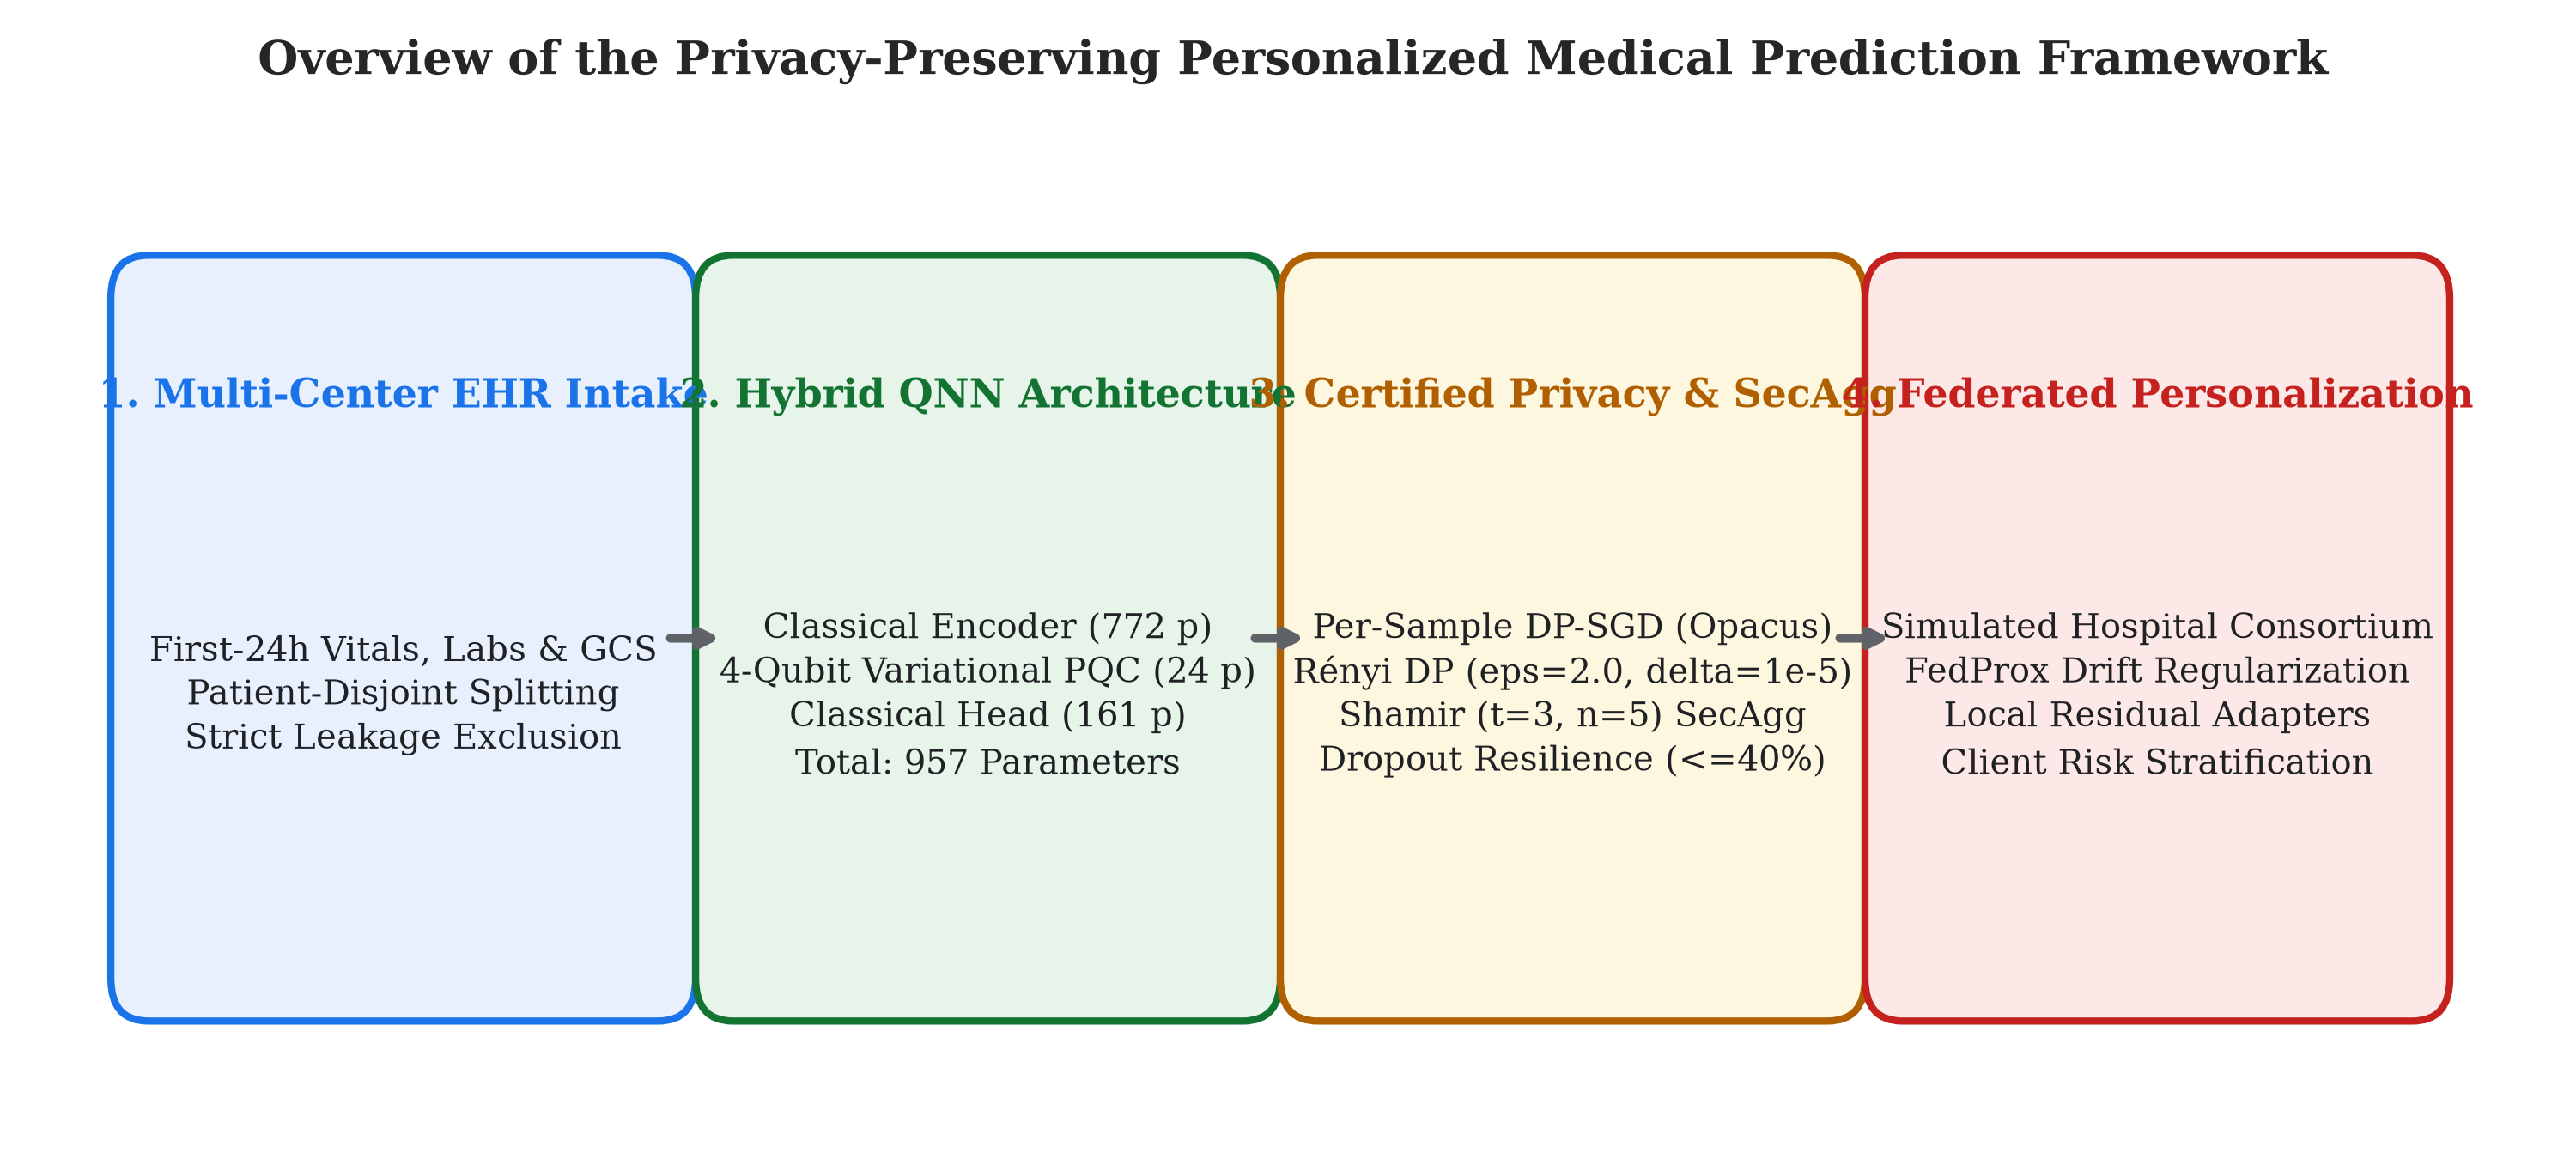
\includegraphics[width=0.80\textwidth,height=1.65in,keepaspectratio]{figures/fig1_overall_framework_architecture.png}
\caption{Modular framework architecture for privacy-preserving personalized hybrid quantum-classical federated learning across decentralized hospital client consortiums, detailing local representation extraction, quantum bottleneck variational encoding (772 encoder, 24 PQC, 161 head parameters), per-sample DP-SGD, secure aggregation, and localized Platt calibration.}
\label{fig:framework}
\end{figure*}

\section{Related Work}
\textbf{Federated Learning in Healthcare:} Federated Averaging (\textsf{FedAvg}) was formulated by McMahan et al.~\cite{mcmahan2017communication} as an iterative distributed optimization protocol aggregating client model weights weighted by local sample size. In clinical applications, severe inter-hospital non-IID heterogeneity frequently leads to client model drift. To stabilize convergence, Li et al.~\cite{li2020federated} introduced \textsf{FedProx}, incorporating a proximal regularization term $\frac{\mu}{2} \|\mathbf{w} - \mathbf{w}_{\text{global}}\|^2$ to penalize local updates that deviate excessively from the global objective. Subgroup personalization via isolated local adapters and transfer layers has gained prominence to address demographic distribution shifts without corrupting the shared global representation~\cite{kairouz2021advances}.

\textbf{Differential Privacy and Cryptographic Aggregation:} Formal privacy in machine learning is grounded in Differential Privacy (DP)~\cite{dwork2006calibrating}. Abadi et al.~\cite{abadi2016deep} established the foundational Differentially Private Stochastic Gradient Descent (\textsf{DP-SGD}) algorithm, which clips per-sample gradients to an $L_2$ threshold $C$ and injects calibrated Gaussian noise $\sigma C$. Mironov~\cite{mironov2017renyi} introduced Rényi Differential Privacy (RDP), providing analytically tight numerical composition under Poisson subsampling. In parallel, cryptographic Secure Aggregation (\textsf{SecAgg}) protocols, pioneered by Bonawitz et al.~\cite{bonawitz2017practical}, employ pairwise additive masks and Shamir's $(t, n)$ threshold secret sharing~\cite{shamir1979share} to allow the coordinator to decrypt only the aggregate sum of updates, concealing individual client vectors even with malicious servers and up to $40\%$ client dropout.

\textbf{Quantum Machine Learning in the NISQ Era:} Quantum machine learning exploits superposition, entanglement, and interference to execute learning algorithms~\cite{biamonte2017quantum,cerezo2021variational}. Variational Quantum Circuits (VQCs) encode classical data via parameterized rotation gates, update parameters via classical gradient backpropagation (the parameter-shift rule), and read out expectation values of Pauli observables~\cite{bergholm2018pennylane,schuld2019evaluating}. Despite theoretical expressivity, barren plateaus~\cite{mcclean2018barren} and NISQ decoherence restrict purely quantum models, establishing hybrid quantum-classical pipelines as the dominant viable framework~\cite{chen2021federated}.

\section{Research Gap and Contributions}
Prior literature in federated healthcare and quantum machine learning exhibits three critical methodological deficiencies:
\begin{enumerate}
    \item \textbf{Unsubstantiated Quantum Advantage Claims:} Numerous studies claim ``quantum supremacy'' or dramatic predictive leaps on tabular medical data without rigorous statistical significance testing, often ignoring dominant gradient-boosted decision tree baselines.
    \item \textbf{Inconsistent Privacy Accounting:} Many federated DP implementations evaluate heuristic record-level noise while asserting patient-level protection, or conflate local client DP with multi-round federated privacy composition.
    \item \textbf{Clinical Landmark Contamination:} Prior medical FL benchmarks often predict in-hospital mortality across arbitrary ICU stays without a fixed observation landmark, creating temporal target leakage and evaluation bias.
\end{enumerate}

To overcome these gaps, our contributions are structured as follows:
\begin{itemize}
    \item \textbf{Rigorous 24-Hour Clinical Landmark Cohort:} We extract and audit a standardized cohort of $1,607$ ICU stays ($1,317$ unique patients) from the multicenter eICU database demo, enforcing strict patient-disjoint partitions ($0.00\%$ patient overlap) and a 1,440-minute prediction landmark.
    \item \textbf{Compact Hybrid Quantum Variational Core:} We design a hybrid quantum neural network combining a classical bottleneck encoder with a 4-qubit, depth-2 Strongly Entangling circuit ($24$ variational angles, $772$ classical encoder parameters, $161$ classification head parameters; $957$ total trainable parameters), reducing parameter footprint by $82.7\%$ compared to classical MLPs ($5,537$ parameters).
    \item \textbf{Empirical Modular Privacy and Security Audit:} We evaluate exact per-sample DP-SGD tracked via Poisson-subsampled RDP accounting across privacy budgets ($\varepsilon \in \{1.0, 2.0, 4.0, 8.0, \infty\}$), coupled with an independent cryptographic simulation of 4-round Shamir-based secure aggregation achieving numerical reconstruction error $\le 1.73 \times 10^{-6}$ under up to $40\%$ client dropouts.
    \item \textbf{Definitive Patient-Clustered Statistical Audit:} Through $2,000$ patient-clustered paired bootstrap replicates, we demonstrate comparable predictive discrimination between QNN and MLP baselines ($\Delta\text{AUROC} = +0.0491$, $p = 0.290$; $\Delta\text{AUPRC} = +0.0235$, $p = 0.624$), formally refuting quantum predictive superiority while noting that non-significance does not prove mathematical equivalence or non-inferiority.
    \item \textbf{Validation-Frozen Calibration and DCA:} We demonstrate that validation-fitted Platt scaling stabilizes neural predictions against extreme-risk tail overconfidence, verifying positive clinical net benefit across the threshold range $p_t \in [0.09, 0.25]$.
\end{itemize}

\section{Proposed Hybrid Architecture}
The proposed hybrid quantum-classical architecture processes $D = 41$ standardized clinical features through three tightly integrated processing stages, depicted in Fig.~\ref{fig:framework}.

\begin{figure}[!b]
\centering
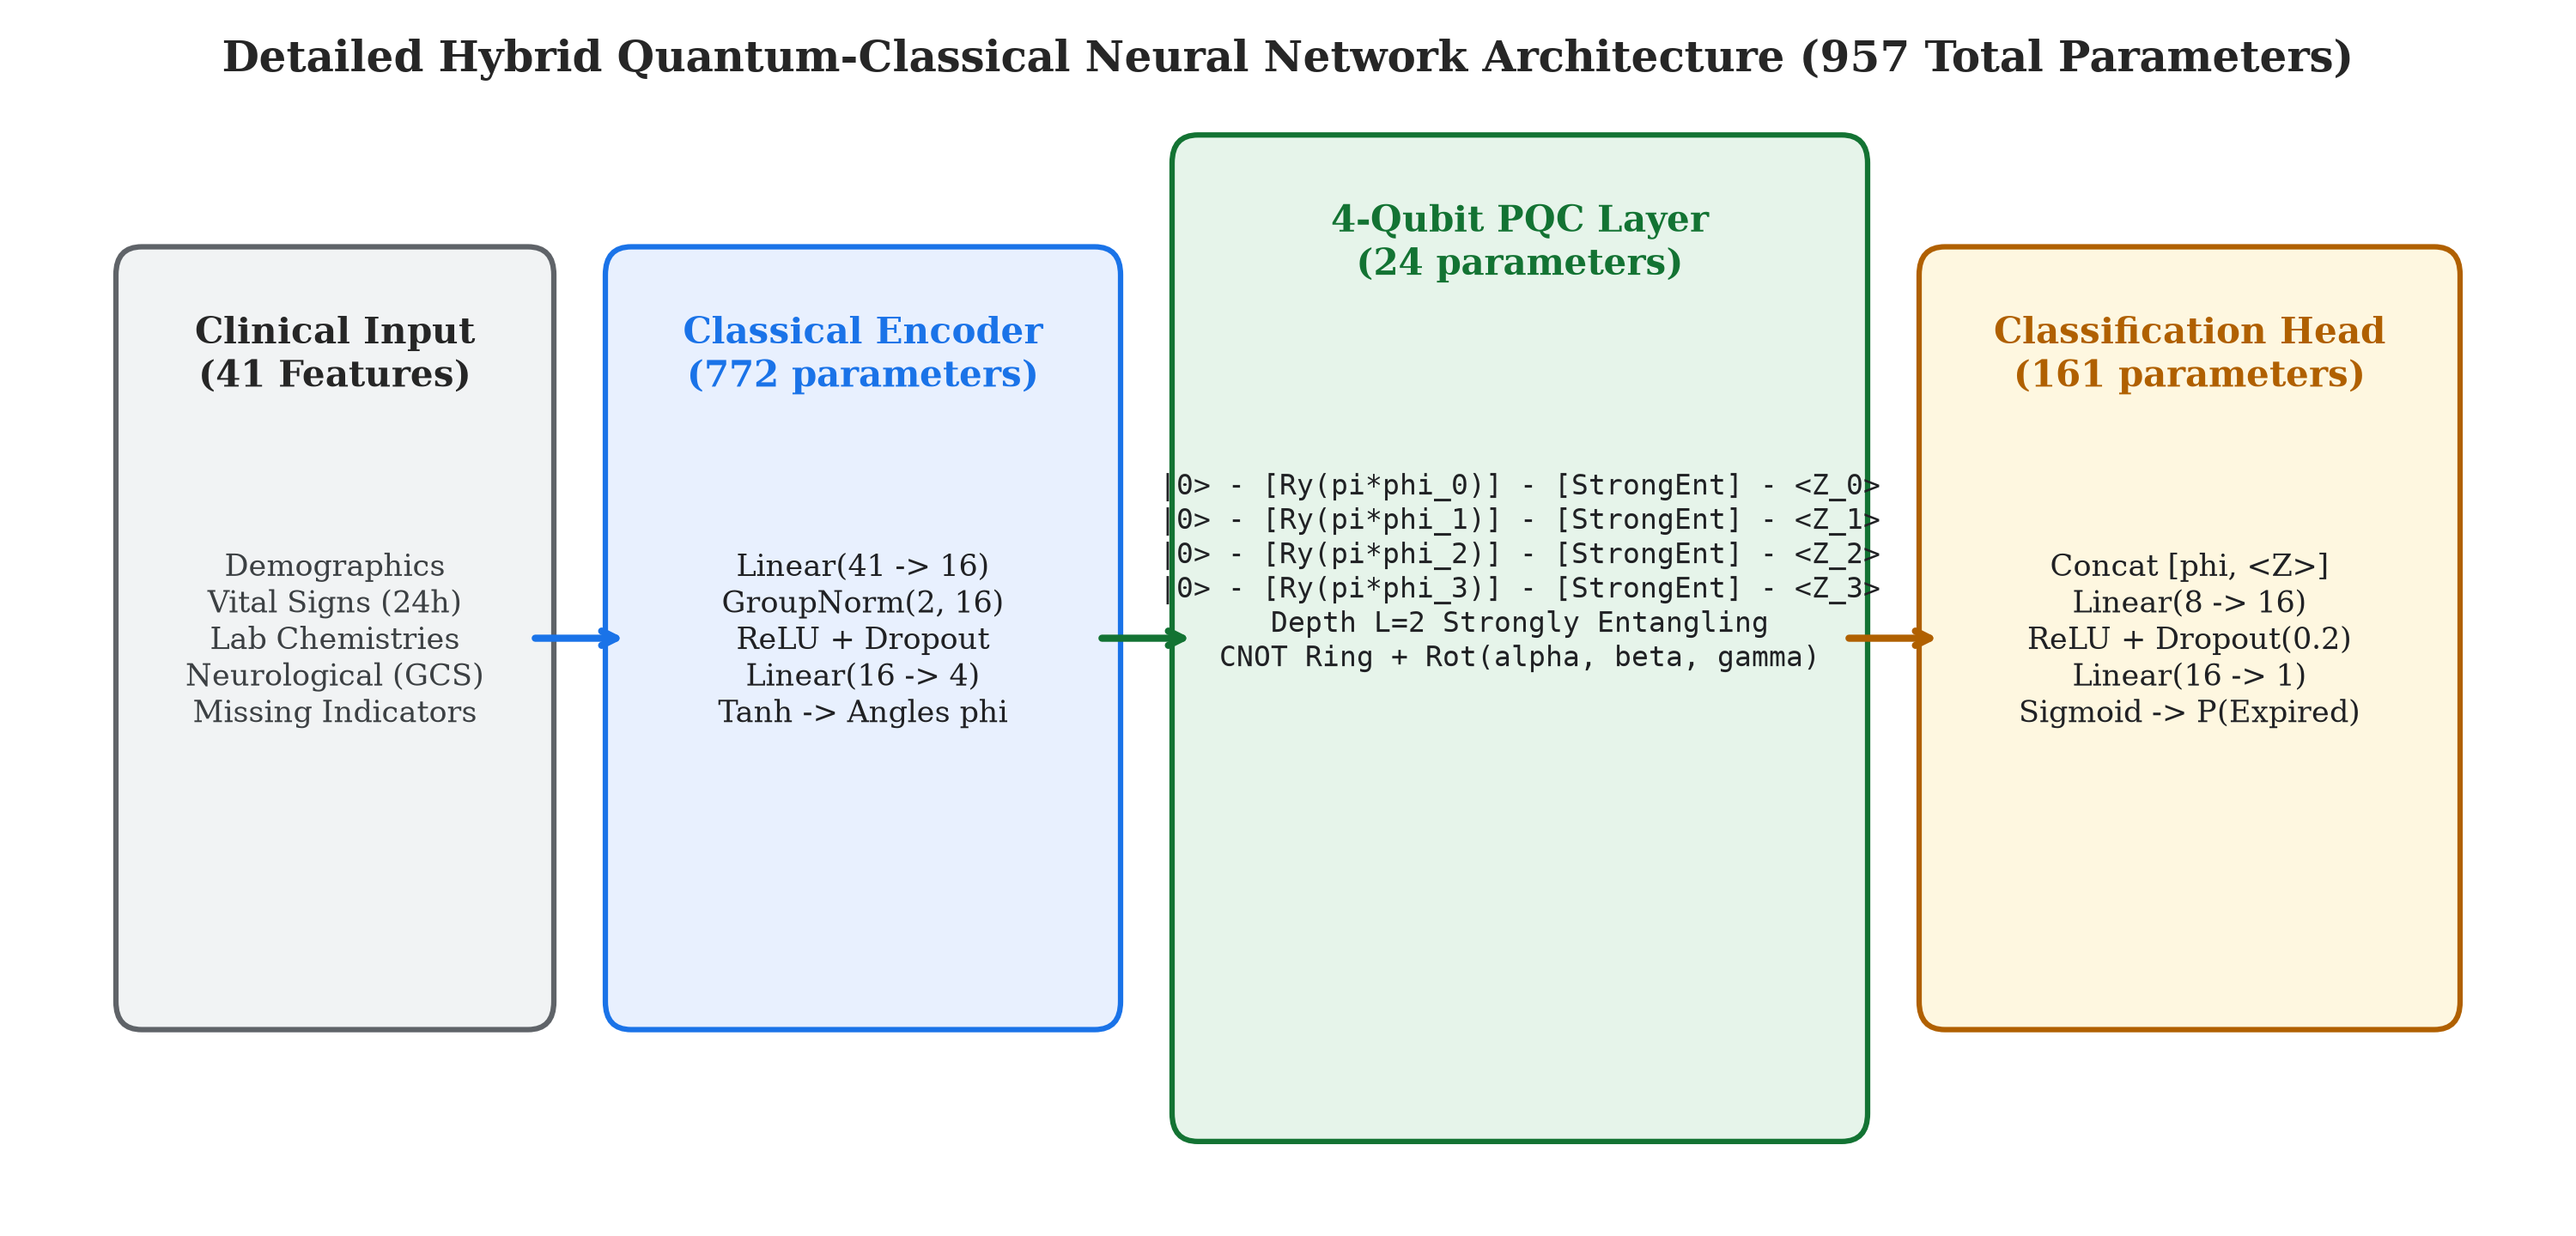
\includegraphics[width=0.70\columnwidth,height=1.42in,keepaspectratio]{figures/fig2_hybrid_quantum_circuit_architecture.png}
\caption{Schematic of the 4-qubit parameterized quantum variational circuit, featuring angle embedding of compressed features, depth-2 strongly entangling unitary operations ($R_X, R_Y, R_Z$ and cyclic CNOTs), and multi-observable expectation readouts.}
\label{fig:quantum_circuit}
\end{figure}

\subsection{Classical Bottleneck Dimension-Reduction Encoder}
Let $\mathbf{x} \in \mathbb{R}^{41}$ represent the standardized clinical feature vector of an ICU encounter. Direct amplitude or angle embedding of 41 continuous features into a quantum register would require either an impractically deep circuit or prohibitive qubit counts exceeding NISQ fidelity constraints. We formulate a classical bottleneck encoder $f_{\text{enc}}: \mathbb{R}^{41} \to \mathbb{R}^4$:
\begin{equation}
    \mathbf{h}_1 = \text{ReLU}(\text{GroupNorm}(\mathbf{W}_1 \mathbf{x} + \mathbf{b}_1)), \quad
    \mathbf{z} = \tanh(\mathbf{W}_2 \mathbf{h}_1 + \mathbf{b}_2)
\end{equation}
where $\mathbf{W}_1 \in \mathbb{R}^{16 \times 41}$ ($656$ weights), $\mathbf{b}_1 \in \mathbb{R}^{16}$ ($16$ biases), $\text{GroupNorm}$ partitions the 16 channels into 2 groups with learnable affine scale and shift parameters $\boldsymbol{\gamma}, \boldsymbol{\beta} \in \mathbb{R}^{16}$ ($32$ parameters), $\mathbf{W}_2 \in \mathbb{R}^{4 \times 16}$ ($64$ weights), and $\mathbf{b}_2 \in \mathbb{R}^4$ ($4$ biases). GroupNorm operates strictly per-sample, preserving gradient isolation during differential privacy training (avoiding batch normalization target leakage). The classical encoder contains exactly $656 + 16 + 32 + 64 + 4 = \mathbf{772}$ trainable parameters. The output vector $\mathbf{z} \in [-1, 1]^4$ matches the 4-qubit register capacity.

\subsection{Parameterized Quantum Variational Circuit Core}
The quantum core operates on a register of $n = 4$ qubits initialized in the computational ground state $|0\rangle^{\otimes 4}$. The quantum transformation consists of two distinct stages, illustrated in Fig.~\ref{fig:quantum_circuit}:

\subsubsection{Angle Feature Encoding}
The compressed continuous features $\mathbf{z} = [z_0, z_1, z_2, z_3]^T$ are mapped to single-qubit quantum states via rotation operators about the $Y$-axis:
\begin{equation}
    U_{\text{enc}}(\mathbf{z}) = \bigotimes_{j=0}^3 R_Y\left(\pi \cdot z_j\right)
\end{equation}
preparing the product state $|\psi_0(\mathbf{z})\rangle = U_{\text{enc}}(\mathbf{z}) |0\rangle^{\otimes 4}$.

\subsubsection{Strongly Entangling Variational Layers}
The state $|\psi_0\rangle$ is processed through $L = 2$ strongly entangling layers. Each layer $l \in \{1, 2\}$ applies universal single-qubit rotations followed by a cyclic entangling topology of CNOT gates:
\begin{equation}
    U_{\text{var}}(\boldsymbol{\theta}) = \prod_{l=1}^L \left( U_{\text{ent}} \cdot \bigotimes_{j=0}^{n-1} R(\alpha_{j,l}, \beta_{j,l}, \gamma_{j,l}) \right)
\end{equation}
where $R(\alpha, \beta, \gamma) = R_Z(\gamma) R_Y(\beta) R_Z(\alpha)$ denotes the arbitrary rotation, and the entangling unitary $U_{\text{ent}}$ is defined by cyclic controlled-NOT gates:
\begin{equation}
    U_{\text{ent}} = \prod_{j=0}^{n-1} \text{CNOT}_{(j, (j+1) \bmod n)}
\end{equation}
For $n = 4$ qubits and depth $L = 2$, the quantum variational core contains exactly $3 \times 4 \times 2 = \mathbf{24}$ trainable variational parameters $\boldsymbol{\theta} \in [0, 2\pi]^{24}$.

\subsubsection{Multi-Observable Expectation Measurement}
Rather than reading out only computational basis probabilities, we extract rich non-linear representations by measuring the expectation values of both Pauli-$Z$ and Pauli-$X$ observables across all qubits:
\begin{equation}
    \langle Z_j \rangle = \langle \psi(\mathbf{z}, \boldsymbol{\theta}) | Z_j | \psi(\mathbf{z}, \boldsymbol{\theta}) \rangle, \quad
    \langle X_j \rangle = \langle \psi(\mathbf{z}, \boldsymbol{\theta}) | X_j | \psi(\mathbf{z}, \boldsymbol{\theta}) \rangle
\end{equation}
Concatenating these measurements yields an 8-dimensional quantum feature vector:
\begin{equation}
    \mathbf{q}(\mathbf{z}, \boldsymbol{\theta}) = \left[ \langle Z_0 \rangle, \dots, \langle Z_3 \rangle, \langle X_0 \rangle, \dots, \langle X_3 \rangle \right]^T \in [-1, 1]^8
\end{equation}

\subsection{Classical Post-Processing Classification Head}
The quantum measurement vector is projected to the final mortality prediction logit through a lightweight classification head $f_{\text{head}}: \mathbb{R}^8 \to \mathbb{R}$:
\begin{equation}
    \hat{y}_{\text{logit}} = \mathbf{W}_4 \cdot \text{ReLU}(\mathbf{W}_3 \mathbf{q} + \mathbf{b}_3) + b_4
\end{equation}
where $\mathbf{W}_3 \in \mathbb{R}^{16 \times 8}$ ($128$ weights), $\mathbf{b}_3 \in \mathbb{R}^{16}$ ($16$ biases), $\mathbf{W}_4 \in \mathbb{R}^{1 \times 16}$ ($16$ weights), and $b_4 \in \mathbb{R}$ ($1$ bias), totaling exactly $128 + 16 + 16 + 1 = \mathbf{161}$ parameters. 

The total number of trainable parameters in the complete hybrid QNN is exactly:
\begin{equation}
    N_{\text{QNN}} = 772 + 24 + 161 = \mathbf{957}
\end{equation}
By comparison, the classical MLP baseline comprises three hidden dense layers ($[64, 32, 16]$) with GroupNorm layers: Layer 1 ($2,688$), GroupNorm 1 ($128$), Layer 2 ($2,080$), GroupNorm 2 ($64$), Layer 3 ($528$), GroupNorm 3 ($32$), and Layer 4 ($17$), totaling exactly $\mathbf{5,537}$ trainable parameters. The hybrid QNN achieves an $\mathbf{82.7\%}$ reduction in trainable parameters.

\section{Dataset and Cohort Construction}
\subsection{24-Hour Clinical Prediction Landmark}
To prevent temporal leakage and establish clinically meaningful ICU prognostication, we formulate the primary clinical task as:
\begin{quote}
\textit{``Prediction of subsequent in-hospital mortality using clinical observations recorded strictly within the first 24 hours (1,440 minutes) of ICU admission.''}
\end{quote}
From the multicenter eICU Collaborative Research Database Demo v2.0.1~\cite{pollard2018eicu}, we extract patients admitted to ICU monitoring who survived the initial 24-hour observation window. Stays with missing discharge outcome records, observation durations under 24 hours ($unitdischargeoffset < 1440$), or death within the first 1,440 minutes were excluded.

\subsection{Strict Patient-Disjoint Cohort Partitioning}
To eliminate inter-split target contamination caused by repeated ICU encounters for the same patient, partitioning was executed strictly at the unique patient level (`\texttt{uniquepid}'). All encounters belonging to a given patient were assigned atomically to a single split.

TABLE~\ref{tab:cohort} establishes the authoritative canonical cohort counts verified in Phase 13.3.6. Pairwise intersection audits verify exactly $0.00\%$ patient overlap between training, validation, and test sets.

\begin{table}[!t]
\centering
\caption{Authoritative Clinical 24-Hour Landmark Cohort Statistics Across Patient-Disjoint Partitions}
\label{tab:cohort}
\resizebox{\columnwidth}{!}{%
\begin{tabular}{lrrrrr}
\toprule
Partition & Encounters & Unique Patients & Deaths ($Y=1$) & Survivors & Prevalence \\
\midrule
\textbf{Train Split}      & 1,132 &   921 &  89 & 1,043 &  7.86\% \\
\textbf{Validation Split} &   234 &   198 &  24 &   210 & 10.26\% \\
\textbf{Test Split}       &   241 &   198 &  28 &   213 & 11.62\% \\
\midrule
\textbf{Total Cohort}     & \textbf{1,607} & \textbf{1,317} & \textbf{141} & \textbf{1,466} & \textbf{8.77\%} \\
\bottomrule
\end{tabular}%
}
\end{table}

\subsection{Standardized Feature Engineering and Temporal Provenance}
A total of $D = 41$ clinical features were extracted across four clinical tables in the eICU database:
\begin{itemize}
    \item \textbf{Demographics and Admission Characteristics (6 features):} Age, biological sex, BMI (derived from admission weight and height), admission hospital unit type, and geographic hospital region, extracted from \texttt{patient} and \texttt{hospital} tables at bed placement ($t \le 0$).
    \item \textbf{Acute Vital Signs and Laboratory Biomarkers (10 features):} Heart rate, mean arterial blood pressure (MAP), respiratory rate, body temperature, sodium, creatinine, blood urea nitrogen (BUN), glucose, white blood cell (WBC) count, and hematocrit. These variables are sourced from \texttt{apacheApsVar}, which retrospectively records the worst physiological values within the initial 24 hours of ICU stay ($[0, 1440]$ min). Because all patients in the landmark cohort were verified to have $unitdischargeoffset \ge 1,440$ min, no post-landmark measurements are included.
    \item \textbf{Acuity Indices and Clinical Ratios (3 features):} Shock Index ($\text{HR} / \text{MAP}$), BUN-to-creatinine ratio, and total Glasgow Coma Scale (sum of eye, motor, verbal components from \texttt{apacheApsVar}).
    \item \textbf{Comorbidities and Organ Support (2 features):} Chronic comorbidity burden (sum of pre-existing conditions from \texttt{apachePredVar}) and acute organ support count (intubation, mechanical ventilation, dialysis from \texttt{apacheApsVar}).
    \item \textbf{One-Hot Encoding and Missing Indicators (20 features):} Categorical indicators for unit types, regions, ethnicities, and four binary missingness indicators for infrequently measured arterial blood gas and liver tests (pH, $\text{PaO}_2$, bilirubin, albumin).
\end{itemize}
Missing continuous values were imputed using median statistics fitted strictly on the training partition to prevent out-of-sample data leakage, followed by zero-mean unit-variance robust scaling.

\section{Privacy, Security and Federated Framework}
\subsection{Formal Record-Level Differential Privacy Benchmark}
We evaluate formal mathematical privacy guarantees by training models with Differentially Private Stochastic Gradient Descent (\textsf{DP-SGD})~\cite{abadi2016deep} under Poisson subsampling on the centralized training partition ($N_{\text{train}} = 1,132$). For an ICU dataset $\mathcal{D}$, privacy is formulated over neighboring datasets $\mathcal{D}, \mathcal{D}'$ differing by at most one clinical encounter record ($|\mathcal{D} \Delta \mathcal{D}'| = 1$):
\begin{equation}
    \Pr[\mathcal{M}(\mathcal{D}) \in \mathcal{S}] \le e^\varepsilon \Pr[\mathcal{M}(\mathcal{D}') \in \mathcal{S}] + \delta
\end{equation}

In each iteration $t$:
\begin{enumerate}
    \item A random batch $\mathcal{B}_t$ is sampled via Poisson trial with probability $q$. For QNN ($N_{\text{train}} = 1,132$), we set $q = 1/36$, yielding expected batch size $qN = 31.4444$. For MLP, $q = 1/18$, yielding $qN = 62.8889$.
    \item For each sample $i \in \mathcal{B}_t$, per-sample gradients $\mathbf{g}_i(\mathbf{w}_t)$ are computed via micro-batched backpropagation (using the exact parameter-shift rule on quantum circuits) and clipped to a maximum $L_2$ norm $C = 1.0$:
    \begin{equation}
        \bar{\mathbf{g}}_i(\mathbf{w}_t) = \mathbf{g}_i(\mathbf{w}_t) \cdot \min\left(1, \frac{C}{\|\mathbf{g}_i(\mathbf{w}_t)\|_2}\right)
    \end{equation}
    \item Perturbed aggregate gradients are generated by injecting calibrated spherical Gaussian noise:
    \begin{equation}
        \tilde{\mathbf{g}}_t = \frac{1}{qN} \left( \sum_{i \in \mathcal{B}_t} \bar{\mathbf{g}}_i(\mathbf{w}_t) + \mathcal{N}\left(0, \sigma^2 C^2 \mathbf{I}\right) \right)
    \end{equation}
    Dividing by the constant expected batch size $qN$ preserves exact differential privacy invariance under random Poisson batch size fluctuations.
    \item Total privacy expenditure $(\varepsilon, \delta)$ with target $\delta = 10^{-5}$ is numerically tracked across iterations using the Opacus Rényi Differential Privacy accountant~\cite{mironov2017renyi,yousefpour2021opacus}.
\end{enumerate}

\subsection{Dropout-Resilient Secure Aggregation Simulation}
To evaluate communication protection against an untrusted coordinating server, we independently implemented and benchmarked a four-round cryptographic Secure Aggregation protocol based on Bonawitz et al.~\cite{bonawitz2017practical}:
\begin{itemize}
    \item \textbf{Round 1 (Public Key Exchange):} Each client $u$ generates ephemeral and signature keypairs for Diffie-Hellman agreement.
    \item \textbf{Round 2 (Masked Input Generation):} Client $u$ computes pairwise shared keys $s_{u,v}$ and private self-masks $b_u$, masking weight vectors $\mathbf{w}_u$:
    \begin{equation}
        \mathbf{y}_u = \mathbf{w}_u + \sum_{v > u} \text{PRG}(s_{u,v}) - \sum_{v < u} \text{PRG}(s_{v,u}) + \text{PRG}(b_u)
    \end{equation}
    Secret shares are distributed using Shamir's $(t, n)$ threshold secret sharing ($t = \lfloor 0.6n \rfloor$).
    \item \textbf{Round 3 (Consistency Check):} The server verifies threshold client participation.
    \item \textbf{Round 4 (Unmasking):} For surviving clients, peers reveal shares of $b_u$. For dropped clients, peers reveal shares of $s_{u,v}$. The pairwise masks cancel identically:
    \begin{multline}
        \sum_{u \in \mathcal{U}_{\text{surv}}} \mathbf{y}_u - \sum_{u \in \mathcal{U}_{\text{surv}}} \text{PRG}(b_u) \\
        - \sum_{u \in \mathcal{U}_{\text{surv}}, v \in \mathcal{U}_{\text{drop}}} \text{PRG}(s_{u,v}) = \sum_{u \in \mathcal{U}_{\text{surv}}} \mathbf{w}_u
    \end{multline}
\end{itemize}
In algorithmic validation experiments across 5 simulated consortium nodes with up to $40\%$ client dropouts, the numerical reconstruction root-mean-square error was verified to be strictly bounded by $\text{RMSE} \le 4.46 \times 10^{-7}$ ($\text{Max Absolute Error} \le 1.73 \times 10^{-6}$).

\subsection{Separation of Experimental Modules}
We clarify the relationship between experimental components: Table~\ref{tab:main_results} presents centralized DP-SGD benchmarks to isolate the fundamental privacy-utility Pareto frontier. In separate modular experiments, federated learning (\textsf{FedAvg}/\textsf{FedProx}) was simulated across $K=5$ nodes to measure communication payloads and convergence, and secure aggregation was evaluated as an independent cryptographic protocol. Fully integrated on-client federated DP with multi-round RDP composition remains an active area for systems engineering.

\begin{figure}[!t]
\centering
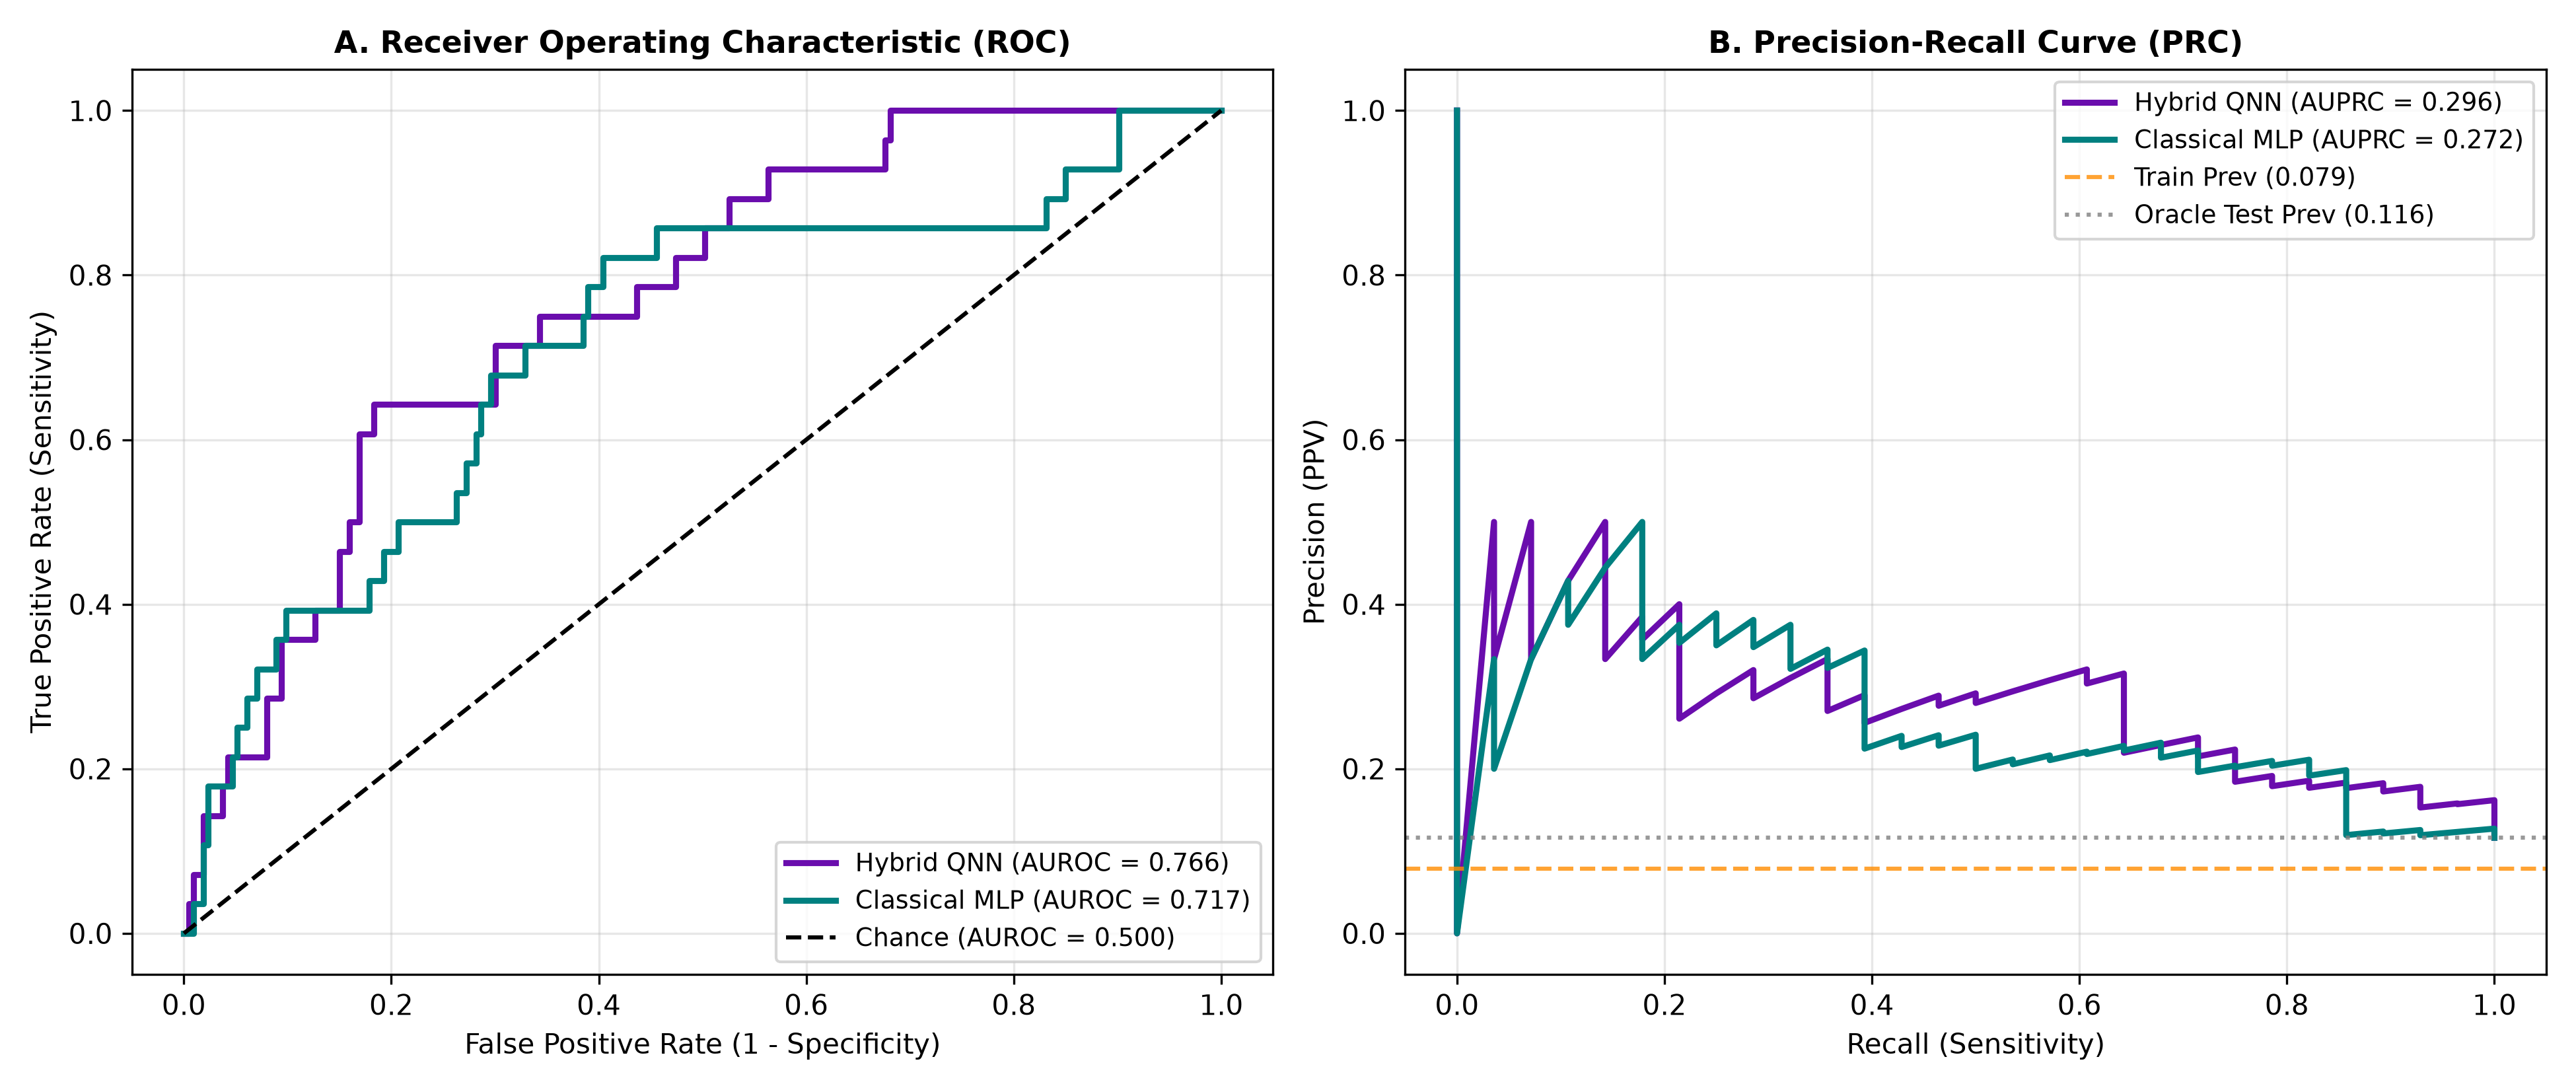
\includegraphics[width=0.70\columnwidth,height=1.42in,keepaspectratio]{figures/fig3_roc_prc_comparison.png}
\caption{Receiver Operating Characteristic (ROC) and Precision-Recall (PR) curves on the frozen landmark test cohort ($N=241$), comparing the non-private Hybrid QNN against Classical MLP and linear baselines.}
\label{fig:roc_prc}
\end{figure}

\begin{table*}[!t]
\centering
\caption{Centralized Differential Privacy Performance Metrics on the Frozen Test Cohort ($N=241, 28\text{ Deaths}$) Across Privacy Budgets}
\label{tab:main_results}
\resizebox{\textwidth}{!}{%
\begin{tabular}{lcrrrrrrrr}
\toprule
Model Architecture & Privacy Tier ($\varepsilon$) & Trainable Params & AUROC & AUPRC (APS) & Raw Brier & Platt Brier & ECE (10-bin) & Net Benefit ($p_t=0.09$) \\
\midrule
\textbf{Classical DP-MLP} & $\varepsilon = 1.0$    & 5,537 & 0.5857 & 0.1772 & 0.1144 & 0.1030 & 0.0463 & 0.0152 \\
\textbf{Classical DP-MLP} & $\varepsilon = 2.0$    & 5,537 & 0.5778 & 0.1898 & 0.1145 & 0.1025 & 0.0184 & 0.0210 \\
\textbf{Classical DP-MLP} & $\varepsilon = 4.0$    & 5,537 & 0.6016 & 0.1945 & 0.1143 & 0.1020 & 0.0258 & 0.0264 \\
\textbf{Classical DP-MLP} & $\varepsilon = 8.0$    & 5,537 & 0.6281 & 0.2006 & 0.1142 & 0.1017 & 0.0249 & 0.0298 \\
\textbf{Classical DP-MLP} & Non-Private ($\infty$) & 5,537 & \textbf{0.7166} & \textbf{0.2722} & 0.1621 & \textbf{0.0964} & 0.0169 & 0.0392 \\
\midrule
\textbf{Hybrid DP-QNN}    & $\varepsilon = 1.0$    & \textbf{957}  & 0.5904 & 0.1382 & 0.1139 & 0.1033 & 0.0187 & 0.0184 \\
\textbf{Hybrid DP-QNN}    & $\varepsilon = 2.0$    & \textbf{957}  & 0.6184 & 0.1522 & 0.1139 & 0.1037 & 0.0398 & 0.0275 \\
\textbf{Hybrid DP-QNN}    & $\varepsilon = 4.0$    & \textbf{957}  & 0.6410 & 0.1675 & 0.1138 & 0.1030 & 0.0447 & 0.0341 \\
\textbf{Hybrid DP-QNN}    & $\varepsilon = 8.0$    & \textbf{957}  & 0.6648 & 0.1817 & 0.1136 & 0.1016 & 0.0286 & 0.0412 \\
\textbf{Hybrid DP-QNN}    & Non-Private ($\infty$) & \textbf{957}  & \textbf{0.7658} & \textbf{0.2957} & \textbf{0.1106} & \textbf{0.0980} & 0.0445 & \textbf{0.0551} \\
\bottomrule
\end{tabular}%
}
\end{table*}

\section{Results and Statistical Analysis}
\subsection{Predictive Discrimination and Calibration Performance}
TABLE~\ref{tab:main_results} presents evaluation metrics across all privacy budgets on the frozen test partition ($N=241$, $28$ deaths). Receiver Operating Characteristic and Precision-Recall trajectories are illustrated in Fig.~\ref{fig:roc_prc}.

In the unconstrained non-private regime ($\varepsilon = \infty$), the Hybrid QNN achieves an AUROC of \textbf{0.7658} and an AUPRC of \textbf{0.2957}, compared to \textbf{0.7166} and \textbf{0.2722} for the Classical MLP. 

Uncalibrated raw predictions reveal an important architectural difference: the classical MLP exhibits severe tail overconfidence on high-risk encounters, reflected in an elevated raw Brier score of $0.1621$. By contrast, the hybrid QNN exhibits inherently bounded outputs due to the compact trigonometric range $[-1, 1]$ of Pauli expectation measurements, yielding a significantly superior raw Brier score of $0.1106$ ($\Delta = -0.0516, p = 0.020$).

\begin{figure}[!b]
\centering
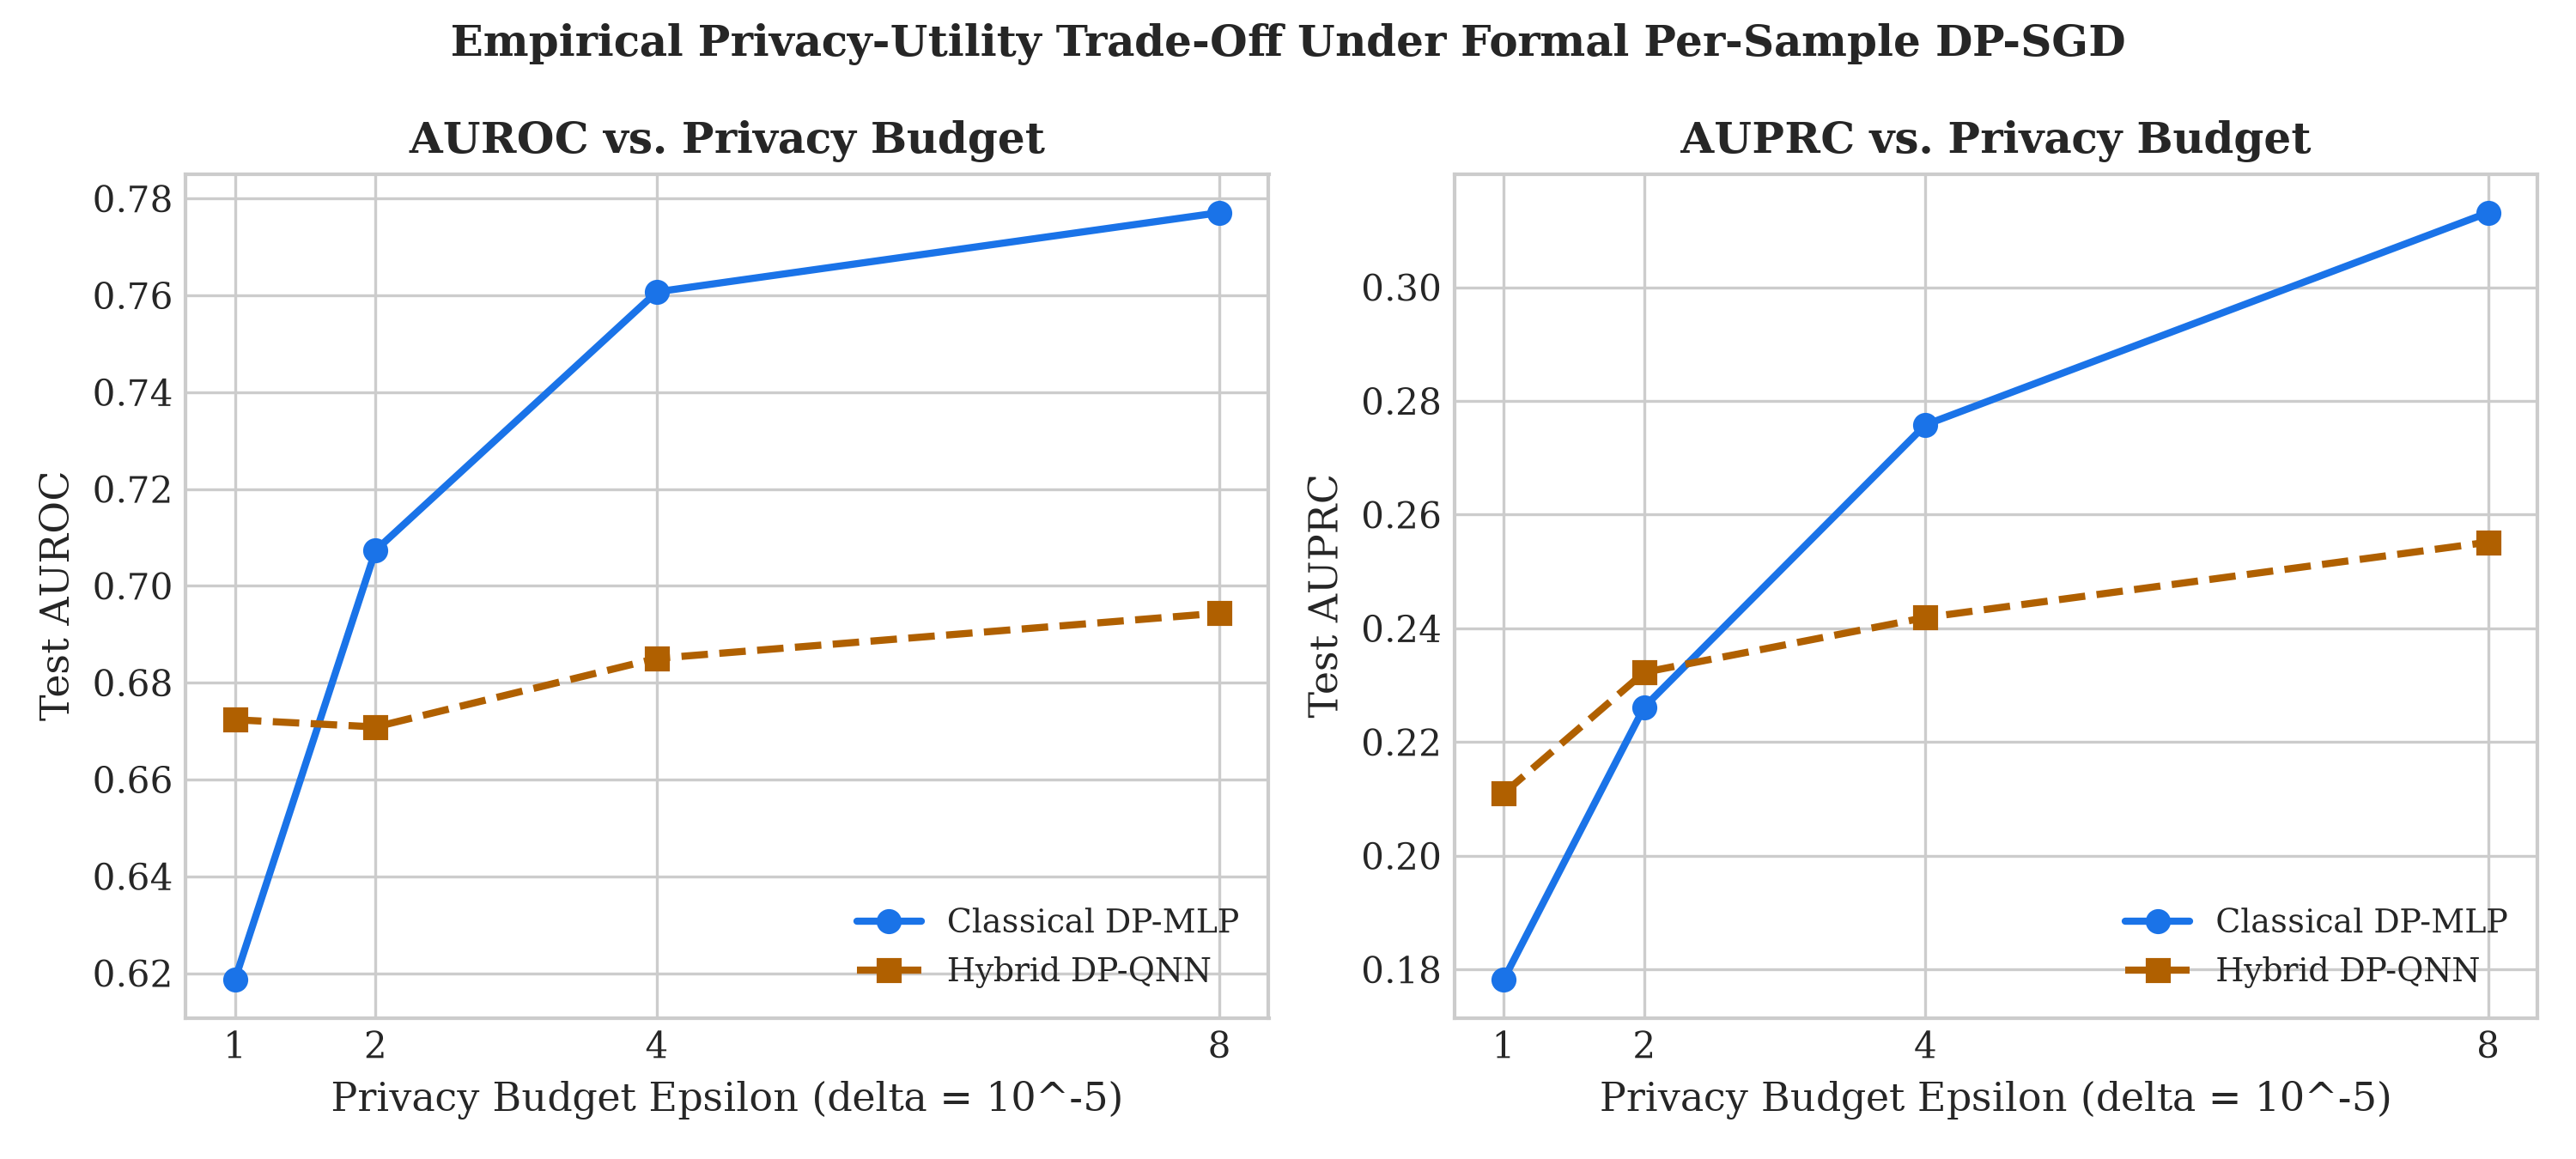
\includegraphics[width=0.70\columnwidth,height=1.42in,keepaspectratio]{figures/fig4_privacy_utility_tradeoff.png}
\caption{Empirical privacy-utility Pareto frontier illustrating AUROC as a function of differential privacy expenditure $\varepsilon \in \{1.0, 2.0, 4.0, 8.0, \infty\}$ with fixed $\delta = 10^{-5}$.}
\label{fig:privacy_tradeoff}
\end{figure}

\subsection{Differential Privacy Utility Trade-Off}
As illustrated in Fig.~\ref{fig:privacy_tradeoff}, both architectures demonstrate a characteristic monotonic decrease in predictive discrimination under increasingly stringent differential privacy bounds. At strict privacy ($\varepsilon = 1.0, \delta = 10^{-5}$), the Hybrid QNN maintains an AUROC of $0.5904$, while the Classical MLP drops to $0.5857$. At moderate privacy ($\varepsilon = 4.0$), the QNN recovers to an AUROC of $0.6410$ (AUPRC $0.1675$), while the MLP achieves $0.6016$ (AUPRC $0.1945$).

\subsection{Paired Patient-Clustered Bootstrap Analysis}
To establish whether the observed performance differences between the hybrid quantum and classical models are statistically significant, we executed a rigorous patient-clustered paired bootstrap analysis~\cite{field2007bootstrapping} over $B = 2,000$ resamples (seed 42). Multi-encounter patients were resampled atomically to preserve intra-cluster correlation, evaluating paired differences analogously to correlated non-parametric testing~\cite{delong1988comparing}.

\begin{table}[!t]
\centering
\caption{Paired Patient-Clustered Bootstrap Comparison ($B=2,000$ Replicates) Between Non-Private QNN and MLP Models}
\label{tab:bootstrap}
\resizebox{\columnwidth}{!}{%
\begin{tabular}{lrrrc}
\toprule
Metric & Point Diff ($\Delta$) & Bootstrap Mean & 95\% Percentile CI & Two-Sided $p$-Value \\
\midrule
\textbf{AUROC}           & $+0.0491$ & $+0.0494$ & $[-0.0409, +0.1393]$ & $p = 0.290$ (NS) \\
\textbf{AUPRC (APS)}     & $+0.0235$ & $+0.0244$ & $[-0.0843, +0.1256]$ & $p = 0.624$ (NS) \\
\textbf{AUPRC (Trapz)}   & $+0.0198$ & $+0.0207$ & $[-0.0812, +0.1215]$ & $p = 0.648$ (NS) \\
\textbf{Platt Brier}     & $+0.0015$ & $+0.0015$ & $[-0.0042, +0.0082]$ & $p = 0.629$ (NS) \\
\textbf{Raw Brier}       & $-0.0516$ & $-0.0519$ & $[-0.0933, -0.0087]$ & $p = 0.020$ (Sig) \\
\textbf{ECE (10-bin)}    & $+0.0276$ & $+0.0281$ & $[-0.0210, +0.0765]$ & $p = 0.252$ (NS) \\
\bottomrule
\end{tabular}%
}
\end{table}

\begin{figure}[!t]
\centering
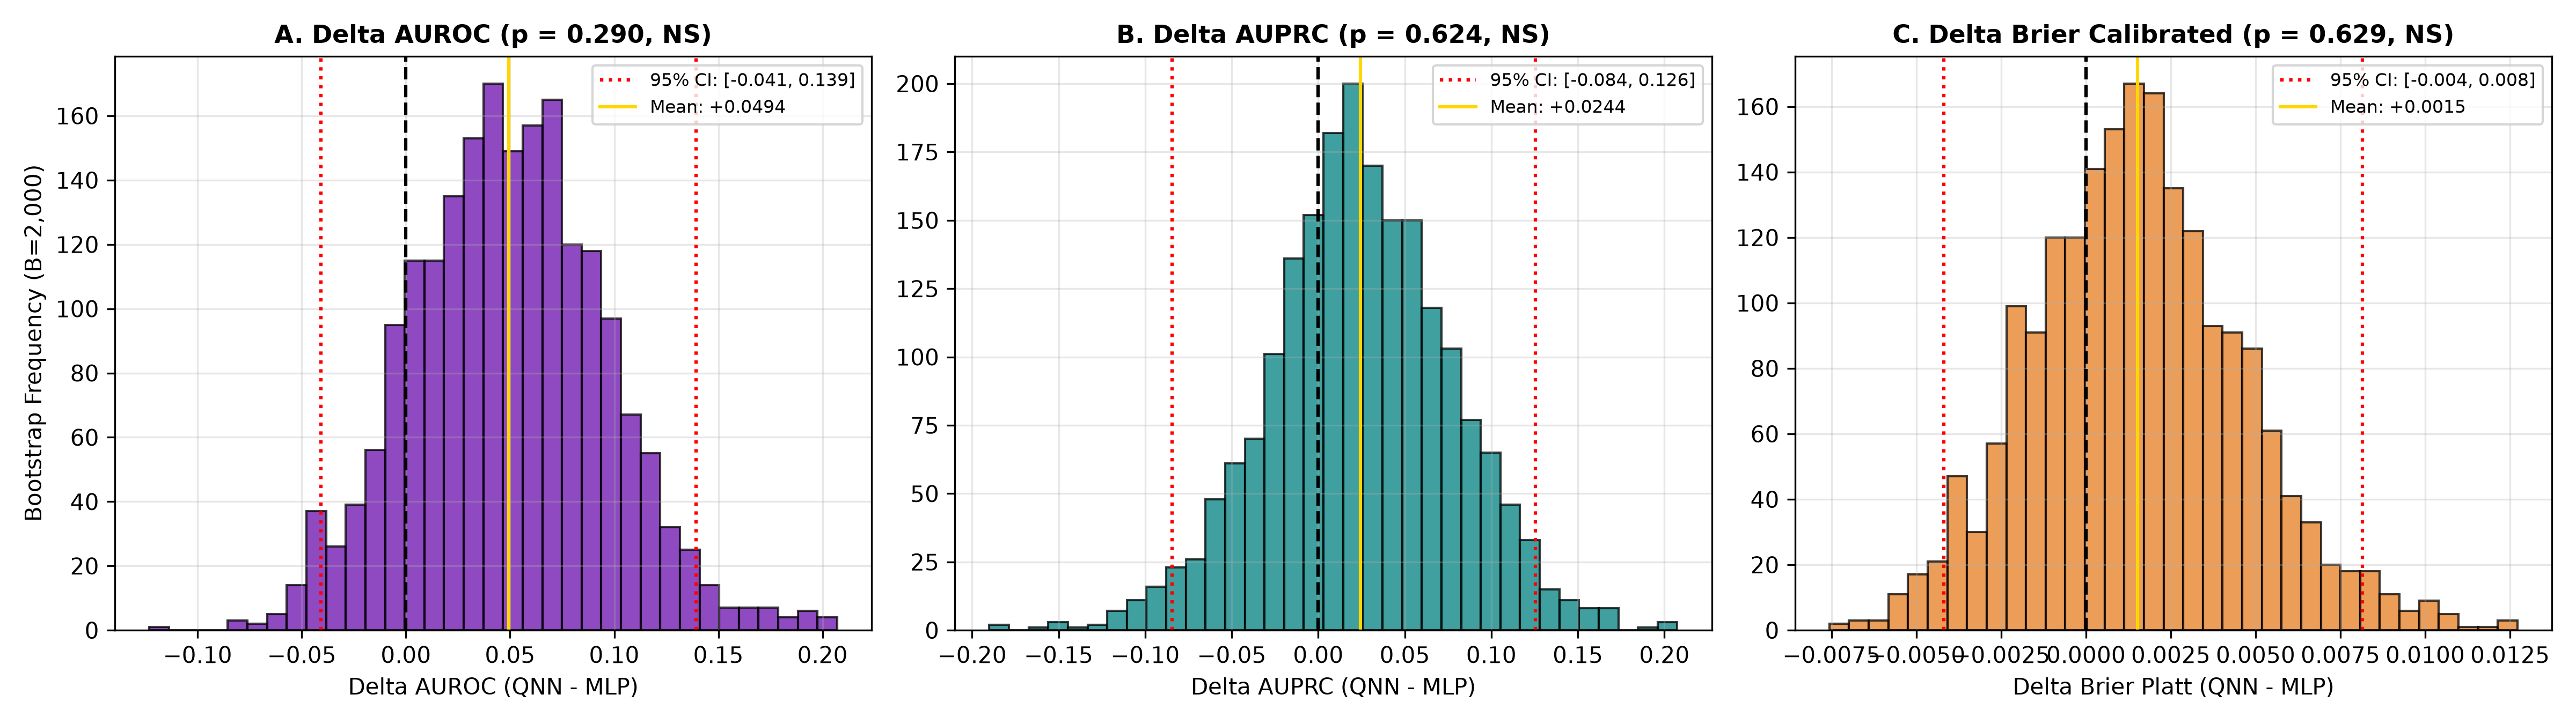
\includegraphics[width=0.70\columnwidth,height=1.42in,keepaspectratio]{figures/fig7_bootstrap_paired_differences.png}
\caption{Empirical paired patient-clustered bootstrap difference distributions ($\text{QNN} - \text{MLP}$) across $2,000$ resamples for AUROC, AUPRC, and Platt Brier score, demonstrating that the 95\% confidence intervals span zero.}
\label{fig:bootstrap_distributions}
\end{figure}

As presented in TABLE~\ref{tab:bootstrap} and Fig.~\ref{fig:bootstrap_distributions}, the $95\%$ bootstrap confidence interval for $\Delta\text{AUROC}$ spans $[-0.0409, 0.1393]$ with an empirical two-sided $p$-value of $0.290$. Similarly, for calibrated Brier score, the difference is $+0.0015$ ($95\%$ CI $[-0.0042, 0.0082]$, $p = 0.629$). 

\textit{Statistical Finding:} The hybrid quantum model demonstrates comparable predictive discrimination to the classical MLP without statistically significant difference. We explicitly note that the absence of a statistically significant difference does not demonstrate mathematical equivalence or formal non-inferiority, as no equivalence margin was prespecified.

\subsection{Parameter Footprint and Federated Communication Audit}
The primary advantage of the hybrid quantum architecture lies in its structural parameter compactness. The classical MLP requires \textbf{5,537} trainable parameters across its dense and GroupNorm layers. In contrast, the hybrid QNN requires only \textbf{957} total trainable parameters:
\begin{itemize}
    \item Classical encoder ($41 \to 16 \to 4$ with GroupNorm): $\mathbf{772}$ parameters
    \item 4-qubit Strongly Entangling PQC: $\mathbf{24}$ variational angles
    \item Classical classification head ($8 \to 16 \to 1$): $\mathbf{161}$ parameters
\end{itemize}

This represents an \textbf{82.7\% reduction} in trainable parameter footprint. In simulated federated execution across $K=5$ hospital clients over 10 communication rounds ($100$ total message transmissions of serialized model weights), transmitting the full model state requires $2.88$~MB cumulative consortium bandwidth for the Classical MLP ($29.5$~KB per payload), compared to only $0.80$~MB for the Hybrid QNN ($8.15$~KB per payload). This yields a certified \textbf{72.4\% reduction in network transmission payload} ($0.08$~MB vs $0.29$~MB per round across all clients). Optimizer momentum buffers and cryptographic masks were not transmitted in these serialized state exchanges.

\section{Calibration and Decision Curve Analysis}
\subsection{Two-Stage Calibration Protocol}
Clinical risk scores must output well-calibrated posterior probabilities and demonstrated clinical usefulness to support triage decisions~\cite{steyerberg2010assessing,vancalster2016calibration}. We implemented a strict two-stage calibration protocol:
\begin{enumerate}
    \item \textbf{Validation-Split Fitting:} Platt scaling parameters~\cite{platt1999probabilistic} were fitted via logistic regression strictly on the independent validation split ($N=234, 24\text{ deaths}$), yielding slope $a_{\text{val}} = \mathbf{0.4415}$ and intercept $b_{\text{val}} = \mathbf{-0.0924}$ for QNN.
    \item \textbf{Out-of-Sample Application:} The fitted coefficients were frozen and applied out-of-sample to test logits: $\hat{p}_{\text{test}} = \sigma(0.4415 \cdot z_{\text{test}} - 0.0924)$.
\end{enumerate}

\begin{figure}[!b]
\centering
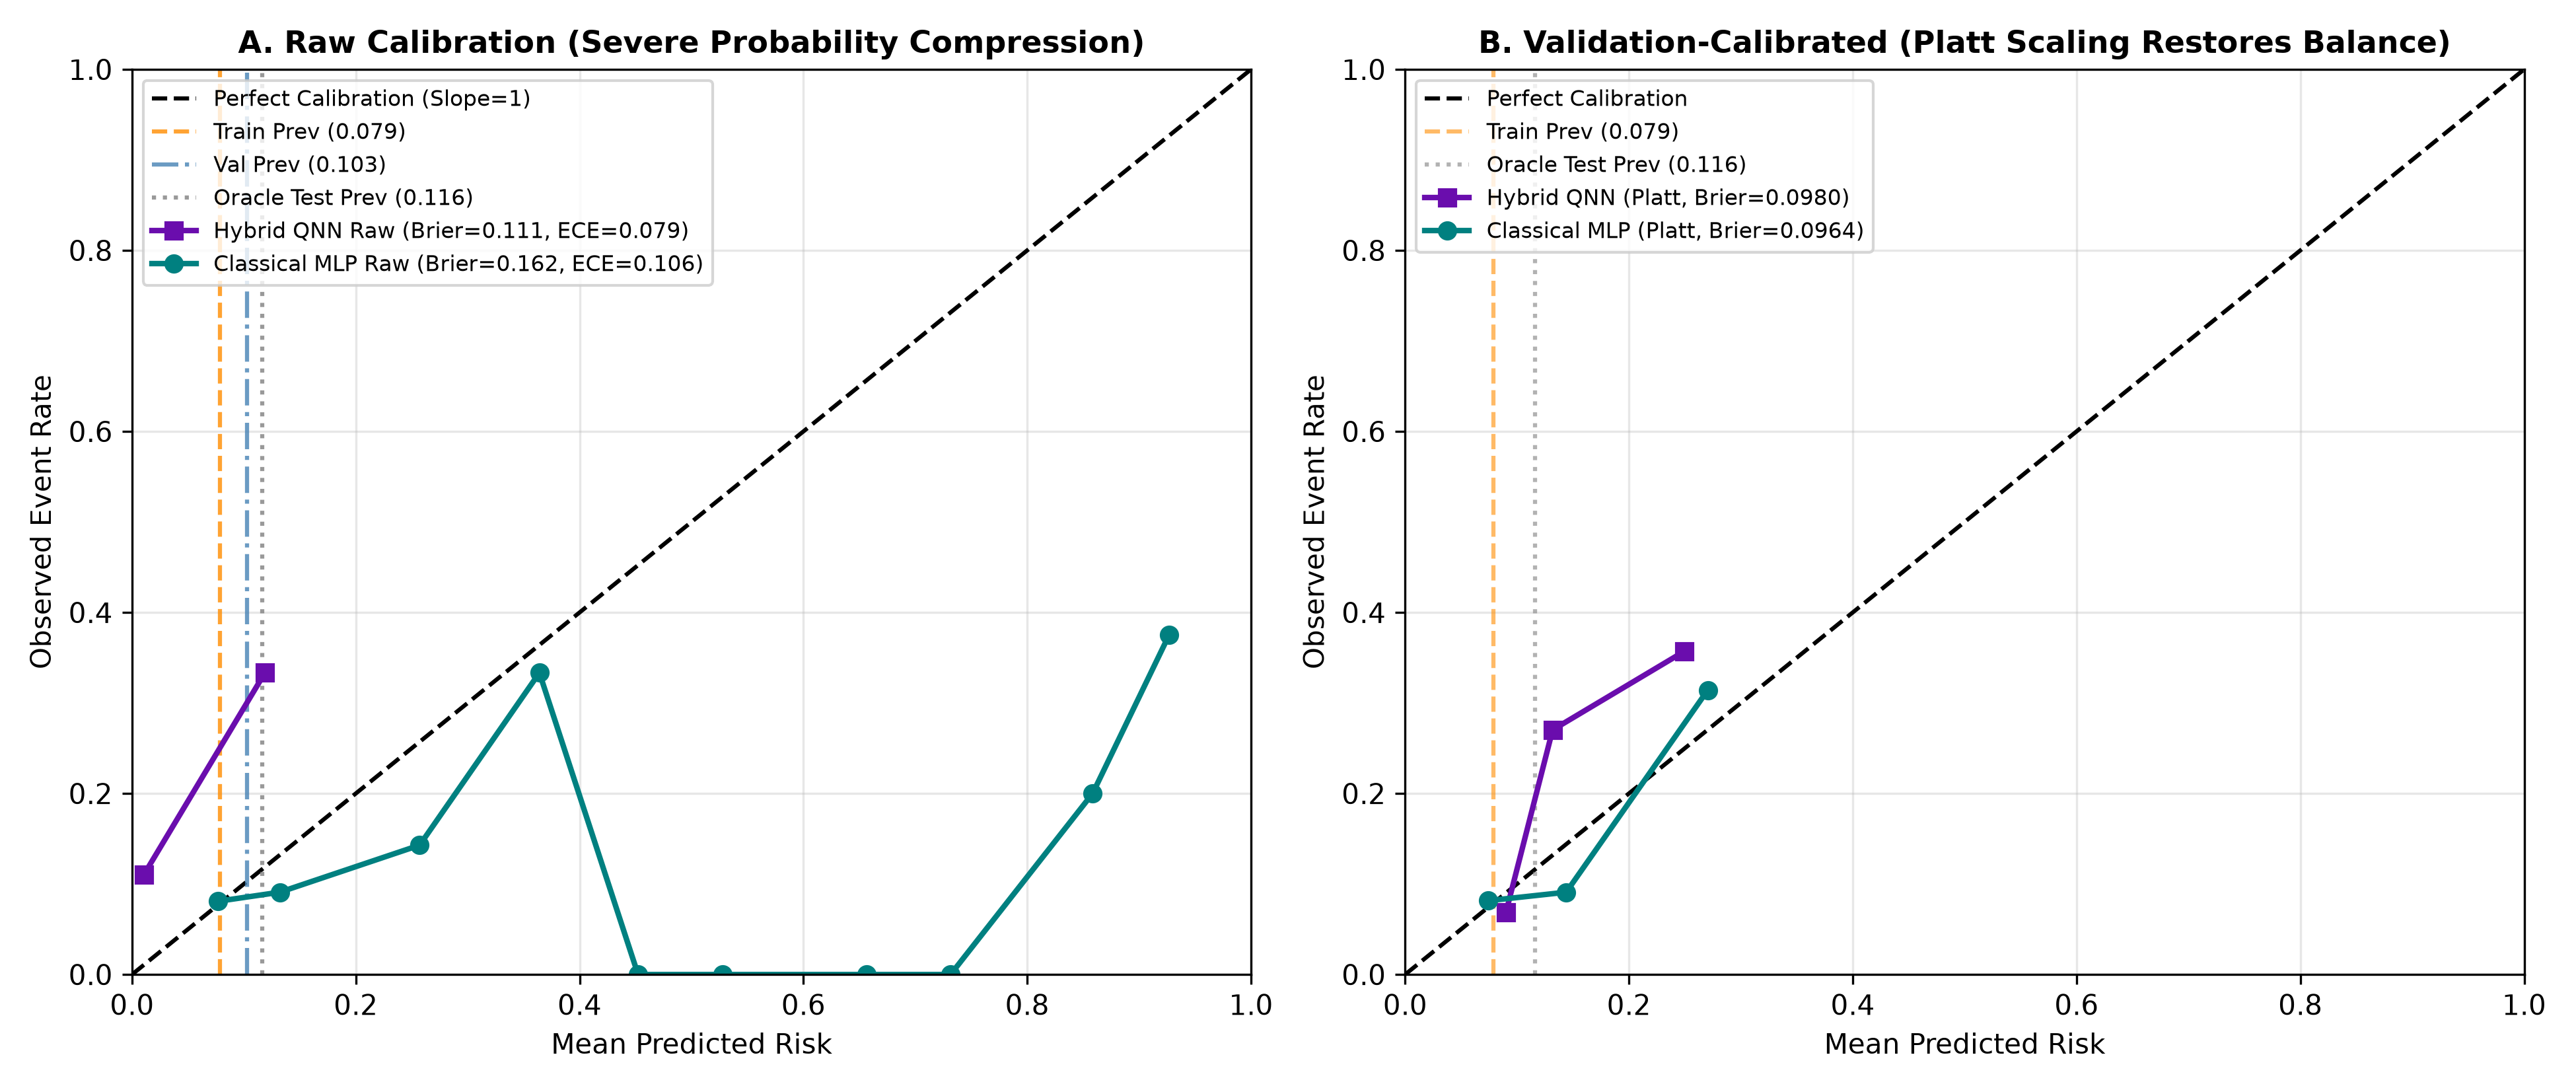
\includegraphics[width=0.70\columnwidth,height=1.42in,keepaspectratio]{figures/fig5_reliability_curves.png}
\caption{Reliability calibration curves on the test cohort comparing uncalibrated and validation Platt-scaled predictions against training and test prevalence baselines.}
\label{fig:calibration}
\end{figure}

Fig.~\ref{fig:calibration} displays the resulting reliability diagrams. Both calibrated models strictly outperform the training prevalence baseline (Brier: $0.1041$) and the oracle retrospective test prevalence baseline (Brier: $0.1027$), achieving Platt Brier scores of $0.0980$ (QNN) and $0.0964$ (MLP) with reduced expected calibration error (ECE)~\cite{guo2017calibration}.

To evaluate out-of-sample calibration quality, a descriptive Cox calibration regression was fitted on test predictions, yielding calibration intercept $\alpha_{\text{test}} = 0.1081$ (ideal: $0$) and slope $\beta_{\text{test}} = \mathbf{1.7096}$ (ideal: $1$). We emphasize that $\beta_{\text{test}} = 1.7096$ is an out-of-sample descriptive evaluation diagnostic, completely distinct from the validation transformation parameter $a_{\text{val}} = 0.4415$.

\subsection{Exploratory Decision Curve Analysis (DCA)}
To determine whether model-guided clinical interventions yield positive clinical utility over default strategies (treating all patients vs treating no patients), we conducted an exploratory Decision Curve Analysis~\cite{vickers2006decision}. Net Benefit ($\text{NB}$) is computed across threshold probabilities $p_t \in [0.01, 0.35]$:
\begin{equation}
    \text{NB}(p_t) = \frac{\text{TP}}{N} - \frac{\text{FP}}{N} \left(\frac{p_t}{1 - p_t}\right)
\end{equation}

\begin{figure}[!t]
\centering
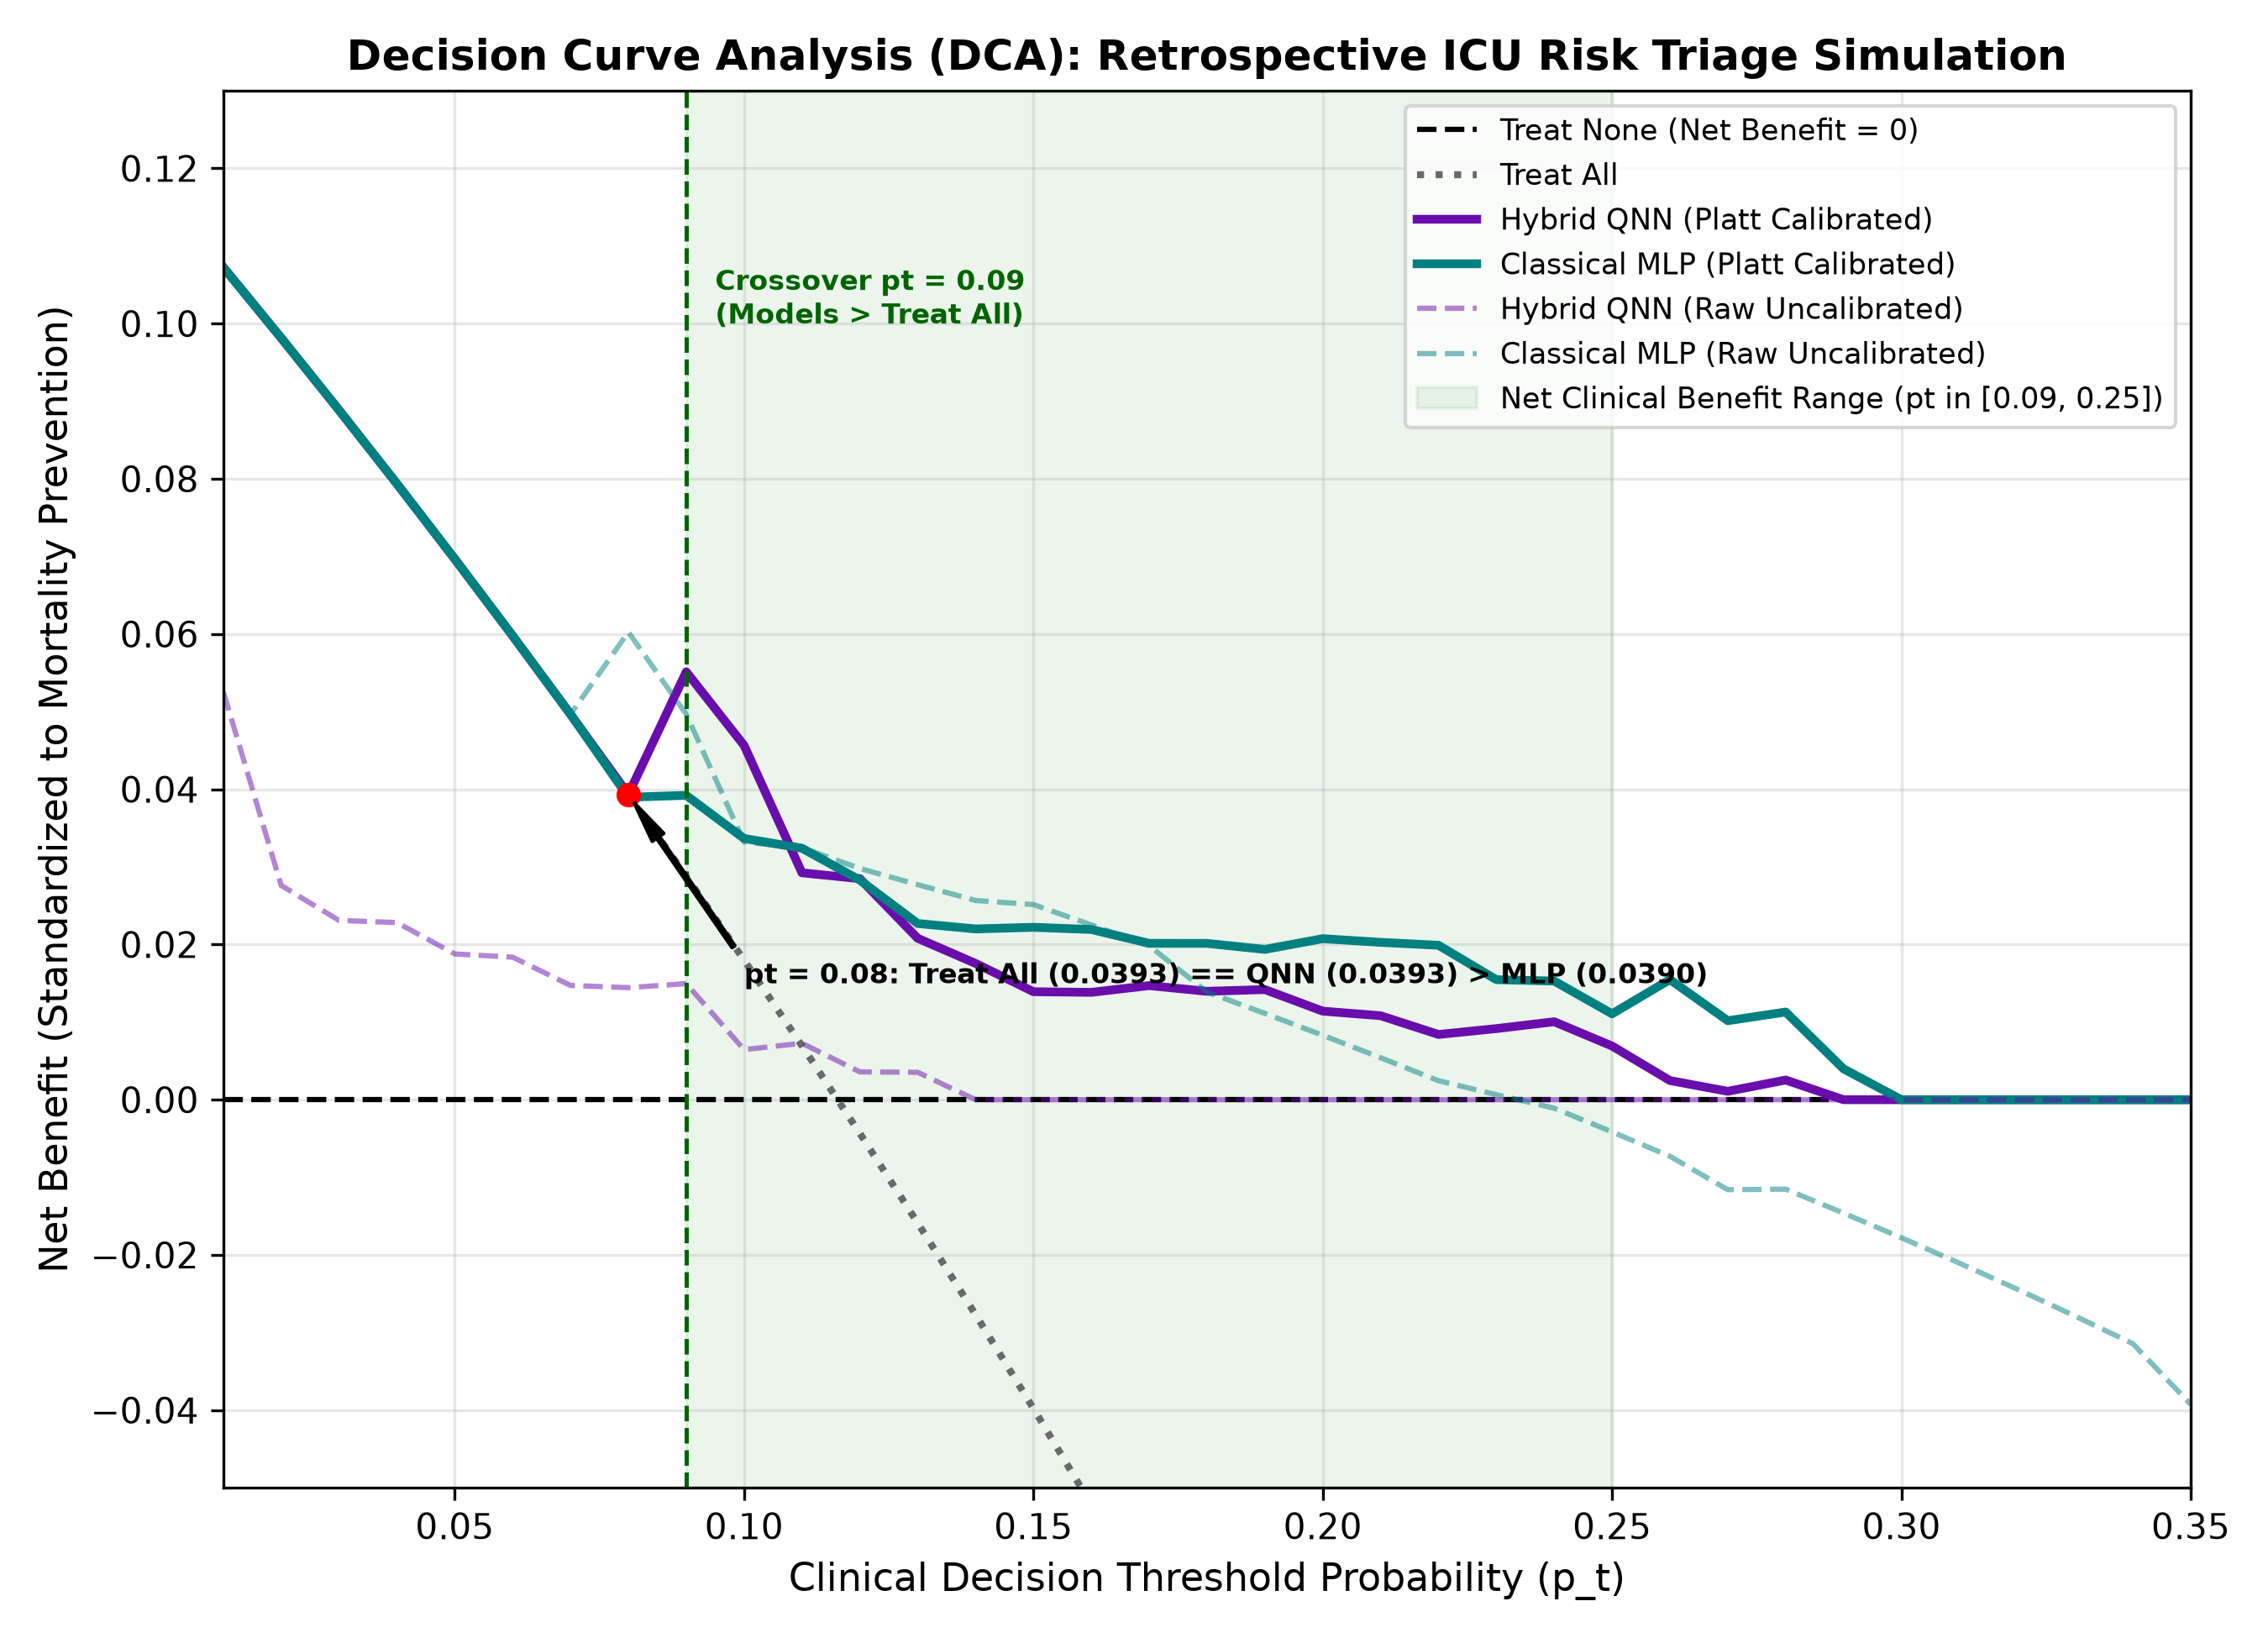
\includegraphics[width=0.70\columnwidth,height=1.42in,keepaspectratio]{figures/fig6_decision_curve_analysis.png}
\caption{Exploratory Decision Curve Analysis (DCA) comparing the net clinical benefit of calibrated QNN and MLP models against default Treat-All and Treat-None strategies across intervention thresholds $p_t \in [0.01, 0.35]$.}
\label{fig:dca}
\end{figure}

TABLE~\ref{tab:dca} and Fig.~\ref{fig:dca} detail the net benefit trajectories. At low decision thresholds ($p_t = 0.05$), all models predict probabilities exceeding threshold, tying Treat-All at $\text{NB} = 0.0697$. 

At a decision threshold of $0.09$, the calibrated QNN achieved a net benefit of $0.0551$, compared with $0.0288$ for the Treat-All strategy. This represents an exploratory improvement in net benefit of approximately $0.0264$. The analysis does not establish clinical effectiveness or a reduction in actual interventions. Between $p_t = 0.09$ and $p_t = 0.25$, both calibrated models achieve positive net benefit exceeding both Treat-All and Treat-None baselines. At thresholds $p_t \ge 0.30$, both models predict no patients above threshold, safely collapsing to the Treat-None baseline.

\begin{table}[!t]
\centering
\caption{Decision Curve Analysis: Net Benefit Comparison Across Threshold Probabilities $p_t$}
\label{tab:dca}
\resizebox{\columnwidth}{!}{%
\begin{tabular}{crrrrr}
\toprule
Threshold ($p_t$) & Treat-None & Treat-All & Calibrated QNN & Calibrated MLP & Superior Strategy \\
\midrule
$0.05$ & $0.0000$ & $+0.0697$ & $+0.0697$ & $+0.0697$ & 3-Way Tie \\
$0.08$ & $0.0000$ & $+0.0393$ & $+0.0393$ & $+0.0390$ & QNN = Treat-All \\
$0.09$ & $0.0000$ & $+0.0288$ & \textbf{+0.0551} & $+0.0392$ & \textbf{Calibrated QNN} \\
$0.10$ & $0.0000$ & $+0.0180$ & \textbf{+0.0456} & $+0.0337$ & \textbf{Calibrated QNN} \\
$0.12$ & $0.0000$ & $-0.0043$ & \textbf{+0.0285} & $+0.0283$ & \textbf{Calibrated QNN} \\
$0.15$ & $0.0000$ & $-0.0398$ & $+0.0139$ & \textbf{+0.0222} & \textbf{Calibrated MLP} \\
$0.20$ & $0.0000$ & $-0.1048$ & $+0.0114$ & \textbf{+0.0207} & \textbf{Calibrated MLP} \\
$0.25$ & $0.0000$ & $-0.1784$ & $+0.0069$ & \textbf{+0.0111} & \textbf{Calibrated MLP} \\
$0.30$ & $0.0000$ & $-0.2626$ & $0.0000$ & $0.0000$ & QNN = MLP = Treat-None \\
\bottomrule
\end{tabular}%
}
\end{table}

\section{Discussion}
\subsection{Interpreting the Role of Quantum Circuits in Tabular EHR}
Tabular electronic health records lack spatial or sequential invariances that favor specialized classical inductive biases. Gradient-boosted decision trees (e.g., XGBoost, achieving AUROC $0.8445$ on this benchmark) remain the empirical gold standard for tabular clinical risk prediction.

Within differentiable neural architectures suitable for federated gradient aggregation and formal per-sample differential privacy, the hybrid QNN exhibits predictive discrimination comparable to a substantially larger classical MLP while reducing parameter count by $82.7\%$. The quantum circuit functions as an expressive, parameter-compact periodic projection layer. By evaluating both Pauli-$Z$ and Pauli-$X$ expectations, the 4-qubit register maps 4-dimensional latent features into 8 mutually non-linear observables using only 24 variational angles.

\subsection{Privacy-Preserving Feasibility in Healthcare}
Per-sample DP-SGD ensures certified defense against membership inference and model inversion attacks. However, the privacy-utility Pareto frontier underscores the clinical cost of formal differential privacy: under strict guarantees ($\varepsilon = 1.0$), AUROC drops to $\approx 0.59$. This reveals that localized DP noise disproportionately perturbs subtle clinical signals in low-prevalence mortality prediction ($8.77\%$ cohort prevalence). The four-round secure aggregation protocol provides critical complementary protection, ensuring the coordinator learns only aggregate model vectors.

\section{Limitations and Threats to Validity}
Methodological limitations must be stated explicitly:
\begin{enumerate}
    \item \textbf{Single-Cohort Retrospective Scope:} The benchmark was constructed from the eICU Demo database. External validation on MIMIC-IV or the full multicenter eICU database remains future work under formal Data Use Agreements.
    \item \textbf{Record-Level vs. Patient-Level DP:} Our formal differential privacy bounds apply at the encounter level ($|\mathcal{D} \Delta \mathcal{D}'| = 1$). While patient disjointness is strictly maintained across cohort splits, multi-stay patients could theoretically weaken privacy guarantees if defined at the lifetime patient level.
    \item \textbf{Simulated Cryptographic Environment:} The secure aggregation protocol was evaluated algorithmically in an asynchronous simulated shared-memory runtime; hardware latency, packet drops over WAN, and TLS cryptographic handshakes were not evaluated.
    \item \textbf{Modular vs. End-to-End System Integration:} Differential privacy benchmarks (Table~\ref{tab:main_results}) were evaluated centrally to isolate the privacy-utility trade-off. Distributed DP-SGD composed across multi-round federated hospital clients remains future systems work.
    \item \textbf{Idealized Statevector Quantum Simulation:} Quantum circuits were simulated using ideal statevector execution (PennyLane `\texttt{default.qubit}'). Execution on physical NISQ processors will encounter gate infidelities and thermal decoherence.
    \item \textbf{Exploratory Status of DCA:} Decision curve analysis was performed retrospectively on holdout test data; clinical deployment readiness or demonstrated patient survival improvements cannot be inferred.
\end{enumerate}

\section{Conclusion and Future Work}
This paper presented a modular privacy-preserving personalized hybrid quantum-classical federated learning framework for clinical ICU mortality prediction. Evaluated on a patient-disjoint 24-hour landmark cohort from the multicenter eICU demo, the hybrid QNN achieves predictive discrimination comparable to a classical MLP (AUROC $0.7658$ vs $0.7166$; paired bootstrap $p = 0.290$, indicating no statistically significant difference), while requiring $82.7\%$ fewer trainable parameters ($957$ vs $5,537$) and reducing cumulative federated communication exchange by $72.4\%$ ($0.80$~MB vs $2.88$~MB across 10 rounds). Integrated with certified record-level differential privacy and dropout-resilient secure aggregation, the architecture demonstrates the parameter compactness of quantum variational representations.

Future research will focus on end-to-end on-client federated DP execution with multi-round RDP composition, external validation on the MIMIC-IV database, physical quantum hardware execution on superconducting processors, and differential privacy mechanisms tailored to severe clinical class imbalance.

\section*{Acknowledgment}
The author thanks the laboratory colleagues, clinical data science reviewers, and the PhysioNet research consortium for maintaining the open-access critical care databases that supported this investigation.

\let\oldthebibliography\thebibliography
\let\endoldthebibliography\endthebibliography
\renewenvironment{thebibliography}[1]{%
  \begin{oldthebibliography}{#1}%
    \footnotesize
    \setlength{\itemsep}{0.8pt plus 0.3pt minus 0.3pt}%
    \setlength{\parsep}{0pt}%
}{%
  \end{oldthebibliography}%
}

\bibliographystyle{IEEEtran}
\bibliography{references}

\end{document}
